% Provenance (never printed): see sources/outline_sources.md (Year 1: fault types and
% Anderson's theory; fold geometry and classification; foliation, schistosity and
% lineation; microstructures). Exercise and problem values in the Book 3 scratch calculator
% calc/ch17.py; the Varden Hills fold and fault from figdata/shared/region.py (read only).
% Fold, anticline, syncline and fold axis are owned by ch. 4; throw and heave by ch. 5;
% trend and plunge by ch. 6; the stresses and the Coulomb criterion by ch. 16. Shear zones
% and deformation mechanisms belong to the Year 3 volume (told here).
\chapter{الصدوع والطيّات والنسيج الصخري}\label{ch:b1:faults-folds-fabrics}

طريق يقطع صخرًا يُظهر وجهًا مصقولًا كالزجاج ومخدوشًا بخطوط دقيقة متوازية. وعبر الوادي، يُظهر جرف بحري طبقات من الحجر الرملي والصفحي ملتوية على شكل تعرّجات بجوانب مستقيمة وزوايا حادة. وعلى سقف قريب، تنشقّ الأردواز إلى صفائح سمكها بضعة مليمترات، على مستويات تقطع الطبقات الطينية التي تكوّنت منها. وكلٌّ منها سجلٌّ لتشوّه الصخر، مقروء على مقياس مختلف: فالخدوش تعطي الاتجاه الذي انزلقت فيه كتلتان متجاوزتين إحداهما الأخرى على امتداد صدع؛ والتعرّجات تقيس مقدار قصر الطبقات؛ والمستويات الأردوازية نمت عبر حبيبات الصخر حين ضُغط. ويقدّم هذا الفصل الهندسة اللازمة لقياس السجلات الثلاثة، وتفسّر ميكانيكا الفصل السابق لماذا تتّخذ الصدوع انحداراتها.

\begin{recall}
\omterm{def:b1:geological-maps:attitude}{وضعية المستوي} هي اتجاه انحداره وانحداره، وتُكتب مثلًا $080/12$؛ ويُستنتج امتداده بقاعدة اليد اليمنى، فالمستوي ينحدر نحو يمين مراقب ينظر على طول \omterm{def:b1:geological-maps:attitude}{الامتداد} (\cref{ch:b1:geological-maps}). 
\omterm{def:b1:geological-maps:fold}{والطيّة} ثنية لطبقات كانت مستوية؛ \omterm{def:b1:geological-maps:fold}{والطية} المحدّبة تكون محدّبة نحو الأعلى وأقدم الصخور في لبّها، \omterm{def:b1:geological-maps:fold}{والطية} المقعّرة مقعّرة نحو الأعلى؛ \omterm{def:b1:geological-maps:fold}{ومحور الطية} هو الخطّ الذي تنثني عنده الطبقات أكثر ما يمكن (\cref{ch:b1:geological-maps}).
\omterm{def:b1:cross-sections:throw}{الإزاحة الرأسية} \omterm{def:b1:cross-sections:throw}{والإزاحة الأفقية} لصدع هما المركّبتان الشاقولية والأفقية لإزاحته (\cref{ch:b1:cross-sections}). وللخطّ اتجاه وغوص، والمتجهة الوحدة النازلة $(\cos p\sin t, \cos p\cos t, -\sin p)$
(\cref{ch:b1:field-lab-methods-1}). الصخر الذي يخضع لمعيار كولوم ينكسر على مستويات تصنع $\ang{45} - \phi/2$ مع $\sigma_1$، والصدوع القائمة تنزلق وفق \omterm{prop:b1:stress-strain-rheology:byerlee}{قانون بايرلي} (\cref{ch:b1:stress-strain-rheology}). \omterm{def:b1:rock-forming-minerals:mineral}{والمعدن} يكون في الانطفاء بين \omterm{def:b1:field-lab-methods-1:microscope}{المستقطِبين المتقاطعين} حين تكون اتجاهات اهتزازه موازية لاتجاهي المستقطِبين (\cref{ch:b1:optical-mineralogy}). وقد لُقيت الصدوع في الكتاب~1، الصف~7؛ والصدوع المعكوسة والدفعات \omterm{def:b1:faults-folds-fabrics:foliation}{والتورّق} في الكتاب~2، الصف~12. والجداء الاتجاهي لمتجهتين عمودي على كلتيهما (الرياضيات، السنة الأولى).
\end{recall}

\section{الصدوع: الهندسة والحركة}\label{sec:b1:faults-folds-fabrics:faults}

الصدع سطح تحرّكت عبره كتلتان من الصخر إحداهما بالنسبة للأخرى. ولوصف الحركة نحتاج إلى أسماء للكتلتين وللإزاحة، وإلى طريقة لقياس اتجاهها داخل مستوى الصدع.

\begin{definition}[الجدار المعلّق، والجدار المرتكز، ومتجهة الانزلاق، والانزلاق الصافي، وزاوية الانزلاق]\label{def:b1:faults-folds-fabrics:fault-elements}
لنفترض أن الصدع مستوٍ محليًّا وغير شاقولي. ف\emph{الجدار المعلّق}\index{الجدار المعلّق} هو الكتلة التي فوقه، و\emph{الجدار المرتكز}\index{الجدار المرتكز} الكتلة التي تحته. ولتكن $A$ نقطة من الجدار المرتكز، و$A'$ النقطة من الجدار المعلّق التي كانت متصلة بها قبل الحركة. و\emph{متجهة الانزلاق}\index{متجهة الانزلاق} $\overrightarrow{AA'}$ هي إزاحة الجدار المعلّق بالنسبة للجدار المرتكز؛ وطولها هو \emph{الانزلاق الصافي}\index{الانزلاق الصافي}. و\emph{زاوية الانزلاق}\index{زاوية الانزلاق} $r$ (وتُسمّى أيضًا الميل الانزلاقي) لمتجهة الانزلاق هي الزاوية المقيسة في مستوى الصدع، من اتجاه \omterm{def:b1:geological-maps:attitude}{الامتداد} المعطى بقاعدة اليد اليمنى إلى متجهة الانزلاق، وهي موجبة حين تشير متجهة الانزلاق إلى أعلى المستوى، وسالبة حين تشير إلى أسفله: $\ang{-180} < r \le \ang{180}$. وهذه اتفاقية علماء الزلازل، تُستعمل ثانيةً للزلازل في \cref{ch:b1:earthquake-source}؛ أما كثير من الجيولوجيين الميدانيين فيسجّلون بدلًا منها زاوية بين 0 و\ang{180}، تُقاس مع عقارب الساعة من \omterm{def:b1:geological-maps:attitude}{الامتداد} مرئيًّا من أعلى، ويضيفون اتجاه الحركة بالكلمات.
\end{definition}
% ledger: ar:rake, ws:rake, ws:fault-terms

سُمّي الجداران باسم التعدين: فالعامل الذي يعمل في عرق مائل كان يقف على \omterm{def:b1:faults-folds-fabrics:fault-elements}{الجدار المرتكز} ويكون \omterm{def:b1:faults-folds-fabrics:fault-elements}{الجدار المعلّق} فوق رأسه. والإزاحة المرئية في قطعة واحدة ليست، في العموم، هي الانزلاق: فطبقة مزاحة على خريطة أو في مقطع تُظهر فصلًا، يتوقف على \omterm{def:b1:geological-maps:attitude}{وضعية} الطبقة. والانزلاق يحتاج إلى نقطتين كانتا واحدة، مثل طرفي خطّ قطعه الصدع، كحافّة عرق صخري عند تماسّه بطبقة.

\begin{omfigure}
\begin{tikzpicture}[>={Stealth[length=5pt]}, font=\small]
% (a) the fault plane seen face-on; slip vector of length 3.6 cm at rake -35 deg
% (normal and sinistral): strike-slip component 3.6 cos 35 = 2.949, dip-slip 3.6 sin 35 = 2.065
\pgfmathsetmacro{\Ls}{3.6*cos(35)}\pgfmathsetmacro{\Ld}{3.6*sin(35)}
\begin{scope}
  \fill[omDef!15] (0,0) rectangle (6.2,3.4);
  \draw[omDef, line width=0.7pt] (0,0) rectangle (6.2,3.4);
  \draw[line width=1.2pt] (0,3.4) -- (6.2,3.4);
  \node[anchor=south, font=\scriptsize] at (3.1,3.4) {خطّ الامتداد، حيث يلتقي الصدع بالأرض};
  \draw[->, line width=0.6pt] (6.45,3.0) -- (6.45,2.0) node[midway, right, font=\scriptsize, align=left] {نزولًا على الانحدار};
  \draw[->, line width=0.6pt] (0.3,0.35) -- (1.3,0.35) node[right, font=\scriptsize] {الامتداد};
  \coordinate (A) at (1.2,2.55);
  \coordinate (B) at ($(A)+(\Ls,0)$);
  \coordinate (A2) at ($(A)+(\Ls,-\Ld)$);
  \draw[omProp, dashed, line width=0.7pt] (A) -- (B) node[midway, above, font=\scriptsize] {مركّبة الانزلاق على الامتداد};
  \draw[omProp, dashed, line width=0.7pt] (B) -- (A2) node[midway, right, font=\scriptsize, align=left] {مركّبة الانزلاق على الانحدار};
  \draw[->, line width=1.3pt, omThm] (A) -- (A2) node[midway, below left, font=\scriptsize, inner sep=1pt] {متجهة الانزلاق};
  \draw[black] ($(A)+(0.9,0)$) arc[start angle=0, end angle=-35, radius=0.9];
  \node[font=\scriptsize] at ($(A)+(-17.5:1.15)$) {$r$};
  \fill (A) circle[radius=1.4pt] node[above left, inner sep=1.5pt] {$A$};
  \fill (A2) circle[radius=1.4pt] node[below right, inner sep=1.5pt] {$A'$};
  \node[font=\small\bfseries] at (3.1,-0.55) {(أ) في مستوى الصدع};
\end{scope}
% (b) the vertical section through the dip line: dip 50 deg; dip-slip 2.065 -> throw 1.582, heave 1.327
\begin{scope}[xshift=9.4cm, yshift=0.2cm]
  \pgfmathsetmacro{\th}{\Ld*sin(50)}\pgfmathsetmacro{\he}{\Ld*cos(50)}
  \fill[omLithSand!40] (-1.2,0) -- (-1.2,3.2) -- (0,3.2) -- ({3.2/tan(50)},0) -- cycle;
  \fill[omLithSand!20] ({3.2/tan(50)},0) -- (0,3.2) -- (4.2,3.2) -- (4.2,0) -- cycle;
  \draw[line width=0.6pt] (-1.2,3.2) -- (4.2,3.2);
  \draw[omDef, line width=1.1pt] (0,3.2) -- ({3.2/tan(50)},0);
  \draw[black] (0.75,3.2) arc[start angle=0, end angle=-50, radius=0.75];
  \node[font=\scriptsize] at ($(0,3.2)+(-25:1.0)$) {$\delta$};
  \coordinate (P) at ({1.3*cos(50)},{3.2-1.3*sin(50)});
  \coordinate (Q) at ($(P)+({\Ld*cos(50)},{-\Ld*sin(50)})$);
  \coordinate (R) at ($(P)+(\he,0)$);
  \draw[->, omProp, line width=1.1pt] (P) -- (Q);
  \draw[black!80, densely dotted, line width=0.7pt] (P) -- (R) node[midway, above, font=\scriptsize] {الإزاحة الأفقية};
  \draw[black!80, densely dotted, line width=0.7pt] (R) -- (Q) node[midway, right, font=\scriptsize] {الإزاحة الرأسية};
  \node[font=\scriptsize, omProp, anchor=east] at ($(P)!0.55!(Q)+(-0.08,0)$) {الانزلاق الشاقولي};
  \node[font=\small] at (3.3,2.6) {الجدار المعلّق};
  \node[font=\small] at (-0.55,1.0) {الجدار المرتكز};
  \node[font=\small\bfseries] at (1.5,-0.75) {(ب) في المستوى الشاقولي للانحدار};
\end{scope}
\end{tikzpicture}
\par\smallskip{\small عناصر الصدع، مرسومة بالمقياس لصدع ينحدر بزاوية $\delta = \ang{50}$ وله \omterm{def:b1:faults-folds-fabrics:fault-elements}{متجهة انزلاق} زاوية انزلاقها $r = \ang{-35}$. (أ) مستوى الصدع من الأمام: تنقسم \omterm{def:b1:faults-folds-fabrics:fault-elements}{متجهة الانزلاق} $\overrightarrow{AA'}$ إلى مركّبة على طول \omterm{def:b1:geological-maps:attitude}{الامتداد} وأخرى نزولًا على \omterm{def:b1:geological-maps:attitude}{الانحدار}. (ب) المقطع الشاقولي العمودي على \omterm{def:b1:geological-maps:attitude}{الامتداد}: تنقسم مركّبة الانزلاق الشاقولي إلى \omterm{def:b1:cross-sections:throw}{الإزاحة الرأسية} \omterm{def:b1:cross-sections:throw}{والإزاحة الأفقية}.}
\label{fig:b1:faults-folds-fabrics:elements}
\end{omfigure}

\begin{proposition}[مركّبات الانزلاق]\label{prop:b1:faults-folds-fabrics:slip-components}
ليكن لصدعٍ اتجاه انحدار $\alpha$ وانحدار $\delta$، ولمتجهة انزلاق طولها $L$ وزاوية انزلاقها $r$. وبمركّبات شرقية وشمالية وعلوية، لتكن $\mathbf s = (\sin(\alpha-\ang{90}), \cos(\alpha-\ang{90}), 0)$ المتجهة الوحدة على طول \omterm{def:b1:geological-maps:attitude}{الامتداد}، و$\mathbf u = (-\cos\delta\sin\alpha,
-\cos\delta\cos\alpha, \sin\delta)$ المتجهة الوحدة صاعدةً على طول \omterm{def:b1:geological-maps:attitude}{الانحدار}. فإن
\[
  \overrightarrow{AA'} = L\,(\cos r\,\mathbf s + \sin r\,\mathbf u),
\]
مركّبتها على \omterm{def:b1:geological-maps:attitude}{الامتداد} هي $L\cos r$، ومركّبتها الشاقولية على \omterm{def:b1:geological-maps:attitude}{الانحدار} $L\sin r$؛ \omterm{def:b1:cross-sections:throw}{والإزاحة الرأسية} هي $L\,|\sin r|\sin\delta$، \omterm{def:b1:cross-sections:throw}{والإزاحة الأفقية} $L\,|\sin r|\cos\delta$، \omterm{def:b1:faults-folds-fabrics:fault-elements}{ومتجهة الانزلاق} تغوص بالزاوية $p$ حيث $\sin p = |\sin r|\sin\delta$.
\end{proposition}

\begin{proof}
المتجهة $\mathbf s$ أفقية وتشير على طول \omterm{def:b1:geological-maps:attitude}{الامتداد}؛ و$\mathbf u$ عكس المتجهة الوحدة النازلة على خطّ \omterm{def:b1:geological-maps:attitude}{الانحدار}، وله اتجاه $\alpha$ وغوص $\delta$ (\cref{ch:b1:field-lab-methods-1}). وكلاهما يقع في مستوى الصدع، و$\mathbf s\cdot\mathbf u = -\cos\delta(\sin(\alpha -
\ang{90})\sin\alpha + \cos(\alpha - \ang{90})\cos\alpha) = -\cos\delta\cos\ang{90} = 0$،
فهما يكوّنان أساسًا متعامدًا معياريًّا لمستوى الصدع. ومتجهة في المستوى طولها $L$ وتصنع الزاوية $r$ مع $\mathbf s$، مقيسة نحو $\mathbf u$، هي
$L(\cos r\,\mathbf s + \sin r\,\mathbf u)$. ومركّبتها الشاقولية هي
$L\sin r\sin\delta$، وحجمها هو \omterm{def:b1:cross-sections:throw}{الإزاحة الرأسية}؛ وجزؤها الأفقي عبر
\omterm{def:b1:geological-maps:attitude}{الامتداد} هو $L\sin r$ مضروبًا في الجزء الأفقي من $\mathbf u$، طوله
$\cos\delta$، وهو \omterm{def:b1:cross-sections:throw}{الإزاحة الأفقية}؛ وجيب غوصها هو مركّبتها الشاقولية مقسومةً على $L$.
\end{proof}

في حالة الصدع الانزلاقي الشاقولي، $|\sin r| = 1$ \omterm{def:b1:cross-sections:throw}{والإزاحة الأفقية} هي \omterm{def:b1:cross-sections:throw}{الإزاحة الرأسية} مقسومةً على $\tan\delta$، كما في \cref{ch:b1:cross-sections}. وتُصنّف \omterm{def:b1:faults-folds-fabrics:fault-elements}{زاوية الانزلاق} الصدوعَ في عائلات.

\begin{definition}[الصدوع العادية والمعكوسة والدفعية والانزياحية ومائلة الانزياح]\label{def:b1:faults-folds-fabrics:fault-types}
صدع يقع متجه انزلاقه على خطّ \omterm{def:b1:geological-maps:attitude}{الانحدار} ($r = \pm\ang{90}$) هو صدع انزلاق شاقولي: \emph{صدع عادي}\index{صدع عادي} حين يهبط \omterm{def:b1:faults-folds-fabrics:fault-elements}{الجدار المعلّق} ($r = \ang{-90}$)، و\emph{صدع معكوس}\index{صدع معكوس} حين يصعد ($r = \ang{90}$). و\emph{الصدع الدفعي}\index{الصدع الدفعي} صدع معكوس ينحدر بزاوية \ang{45} أو أقلّ. وصدع يكون انزلاقه موازيًا لامتداده ($r = 0$ أو \ang{180}) هو \emph{صدع انزياحي}\index{صدع انزياحي}؛ وهذه الصدوع عادةً شبه شاقولية. والصدع الانزياحي \emph{أيمن}\index{أيمن} (انزياح يميني) حين يرى مراقب واقف على أحد جانبيه الجانب الآخر يتحرّك نحو اليمين، و\emph{أيسر}\index{أيسر} (انزياح يساري) حين يتحرّك نحو اليسار. والصدع الذي يملك انزلاقه مركّبة انزياحية ومركّبة شاقولية معًا هو \emph{صدع مائل الانزياح}\index{صدع مائل الانزياح}؛ وعمليًّا يُسمّى الصدع باسم مركّبته الأكبر، \omterm{def:b1:faults-folds-fabrics:fault-elements}{فزاوية الانزلاق} القريبة من \ang{-90} يُسمّى بها الصدع عاديًّا.
\end{definition}
% ledger: usgs:fault-types, ws:fault-terms, ar:rake

\begin{proposition}[معنى الصدع الانزياحي]\label{prop:b1:faults-folds-fabrics:sense}
لا يتوقف معنى \omterm{def:b1:faults-folds-fabrics:fault-types}{الصدع الانزياحي} على الجانب الذي يقف عليه المراقب. \omterm{def:b1:faults-folds-fabrics:fault-elements}{فزاوية الانزلاق} القريبة من $0$ تكون \omterm{def:b1:faults-folds-fabrics:fault-types}{أيسر}، والقريبة من \ang{180} \omterm{def:b1:faults-folds-fabrics:fault-types}{أيمن}.
\end{proposition}

\begin{proof}
إذا رأى مراقب على الكتلة 1 الكتلة 2 تتحرّك بمقدار $\mathbf v$، فإن مراقبًا على الكتلة 2 يرى الكتلة 1 تتحرّك بمقدار $-\mathbf v$. وحين يلتفت المراقب الثاني ليواجه الكتلة 1، يكون قد تبادل اليمين واليسار. فالتغيّران يلغي أحدهما الآخر: فكلاهما يرى الجانب الآخر يتحرّك في الاتجاه نفسه، نحو اليمين أو نحو اليسار. أما الجزء الثاني، فقف على \omterm{def:b1:faults-folds-fabrics:fault-elements}{الجدار المرتكز} وواجه \omterm{def:b1:faults-folds-fabrics:fault-elements}{الجدار المعلّق}: عندئذٍ تنظر نحو أسفل \omterm{def:b1:geological-maps:attitude}{اتجاه الانحدار}، ولأن المستوى ينحدر نحو اليمين من امتداده، فإن اتجاه \omterm{def:b1:geological-maps:attitude}{الامتداد} يشير نحو يسار المرء. وزاوية انزلاق $0$ تحرّك \omterm{def:b1:faults-folds-fabrics:fault-elements}{الجدار المعلّق} على طول \omterm{def:b1:geological-maps:attitude}{الامتداد}، نحو اليسار؛ وزاوية \ang{180} تحرّكه نحو اليمين.
\end{proof}

سطح الصدع نفسه غالبًا سجلٌّ للحركة: فالخدوش والألياف عليه تقع على طول الانزلاق. وحول السطح، قد تملأ منطقة الصدع صخورٌ مكسّرة بالحركة.

\begin{definition}[الخدوش المنزلقة، والسطح المخدَّش، وصخور الصدع]\label{def:b1:faults-folds-fabrics:fault-rocks}
\emph{الخدوش المنزلقة}\index{الخدوش المنزلقة} خدوش أو ألياف على سطح الصدع، موازية للانزلاق؛ و\emph{السطح المخدَّش}\index{السطح المخدَّش} هو سطح صدع يحملها، وكثيرًا ما يُصقله الانزلاق. و\emph{صخر الصدع}\index{صخر الصدع} صخرٌ تكوّن بالحركة على صدع. و\emph{البريشيا الصدعية}\index{البريشيا الصدعية} مؤلّفة من شظايا زاويّة من جدران الصدع، مُدارة ومُزاحة عن موضعها، من كتل ضخمة حتى نحو \qty{2}{mm}؛ و\emph{الكاتاكلازيت}\index{الكاتاكلازيت} مؤلّف من شظايا بحجم الرمل أو أصغر؛ وليس لأيّ منهما نسيج، فالشظايا مرمية عشوائيًّا. و\emph{الطين الصدعي}\index{الطين الصدعي} صخر صدعي غني بالطين، لين جدًّا في \omterm{def:b1:geological-maps:geological-map}{الانكشاف}. و\emph{الميلونيت}\index{الميلونيت} صخر ناعم الحبيبات ذو تورّق قوي، يتكوّن في منطقة قصّ بالقصّ اللدن، وتصغر حبيباته بإعادة التبلور لا بالطحن.
\end{definition}
% ledger: ws:fault-terms, ws:fault-rocks

تحدّد صخور الصدع عمقًا، فهي تتبع \omterm{def:b1:stress-strain-rheology:strength-envelope}{غلاف المتانة} في \cref{ch:b1:stress-strain-rheology}. \omterm{def:b1:faults-folds-fabrics:fault-rocks}{فالطين الصدعي} والبريشيا \omterm{def:b1:faults-folds-fabrics:fault-rocks}{والكاتاكلازيت}، بنسيجها العشوائي، تتكوّن بالانزلاق الاحتكاكي والكسر في \omterm{def:b1:layered-earth:layers}{القشرة} الهشّة؛ والميلونيتات تتكوّن تحت \omterm{def:b1:stress-strain-rheology:strength-envelope}{الانتقال الهشّ--اللدن}، حيث يستمرّ الصدع إلى الأسفل كنطاق من القصّ اللدن. وبالنسبة لمنحنى حراري عادي ومياه كافية، ينحصر الانتقال بين الاثنين عند \qtyrange{10}{15}{km}، قريبًا من \qty{13.7}{km} من غلاف الفصل السابق، والصدع أقوى ما يكون هناك. وعبر صدع كبير أُصعد من العمق، يُرى الترتيب نفسه جنبًا إلى جنب: مناطق طين صدعي قرب السطح، ثم \omterm{def:b1:faults-folds-fabrics:fault-rocks}{الكاتاكلازيت}، ثم \omterm{def:b1:faults-folds-fabrics:fault-rocks}{الميلونيت}. وتسمية \omterm{def:b1:faults-folds-fabrics:fault-rocks}{الميلونيت}، المأخوذة من الكلمة اليونانية لطحن الدقيق، تحفظ خطأً: فقد ظُنّ أنه صخر مطحون. ويدرس مجلد السنة الثالثة تلك الأقواس القصّية العميقة والآليات التي تُكوّن الميلونيتات.
% ledger: sibson:fault-rocks, sibson:alpine-fault, ws:fault-rocks

\begin{omfigure}
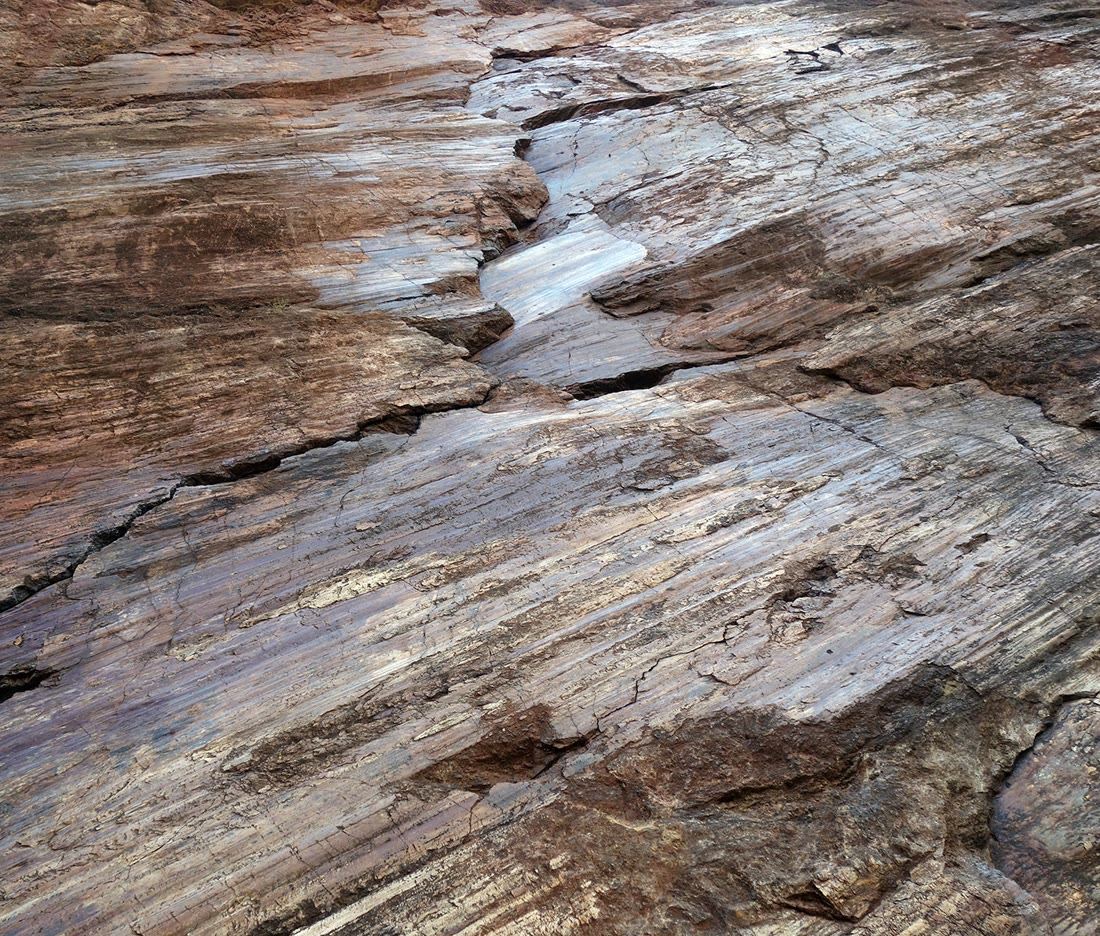
\includegraphics[height=5.2cm]{images/book3/b1-slickenside.jpg}\hfill
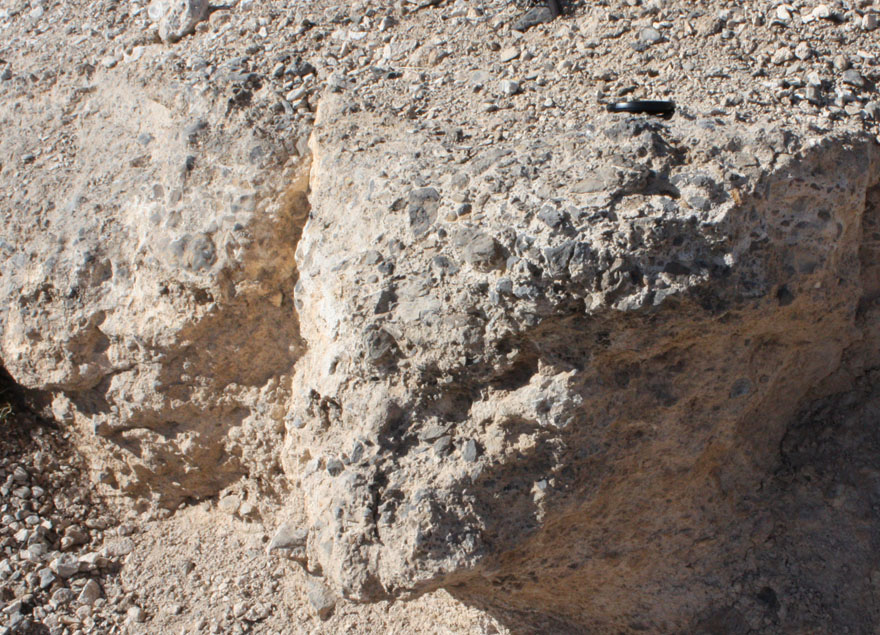
\includegraphics[height=5.2cm]{images/book3/b1-fault-breccia.jpg}
\par\smallskip{\small يسارًا: سطح مخدّش على سطح صدع في الصوّان، بمساحة نحو \qtyproduct{3 x 3}{m} من سطح ارتفاعه \qty{10}{m}، في تلال كورونا هايتس، سان فرانسيسكو؛ والوجه المصقول مخطّط على طول الانزلاق. تصوير: Dextersinister, CC~BY-SA~4.0. ويمينًا: بريشيا صدعية من \omterm{def:b1:faults-folds-fabrics:fault-types}{الصدع الدفعي} كيستون، في كانيون ريد روك، نيفادا: شظايا زاوية من صخر كربوناتي رمادي في مادة أفتح؛ وغطاء العدسة في أعلى اليمين عرضه \qty{5.8}{cm}. تصوير: Jstuby, ملك عام. وكلتاهما من ويكيميديا كومنز.}
\label{fig:b1:faults-folds-fabrics:fault-surfaces}
\end{omfigure}
% ledger: commons:slickenside, commons:breccia

\begin{method}[قياس الانزلاق على صدع]\label{met:b1:faults-folds-fabrics:slip}
\begin{enumerate}
  \item قِس \omterm{def:b1:geological-maps:attitude}{وضعية} سطح الصدع $\alpha/\delta$، واكتب امتداده، $\alpha - \ang{90}$.
  \item قِس \omterm{def:b1:faults-folds-fabrics:fault-rocks}{الخدوش المنزلقة}: زاوية انزلاقها على الصدع، أو اتجاهها وغوصها؛ ومن أجل زاوية انزلاق $r$، $\sin p = |\sin r|\sin\delta$.
  \item اعرف في أيّ اتجاه تحرّك \omterm{def:b1:faults-folds-fabrics:fault-elements}{الجدار المعلّق}، من علامات مزاحة عبر الصدع، وأعطِ \omterm{def:b1:faults-folds-fabrics:fault-elements}{زاوية الانزلاق} إشارتها: سالبة إن هبط \omterm{def:b1:faults-folds-fabrics:fault-elements}{الجدار المعلّق}.
  \item أوجد \omterm{def:b1:faults-folds-fabrics:fault-elements}{الانزلاق الصافي} $L$ من نقطتين كانتا واحدة؛ وإن لم تُعرف إلا \omterm{def:b1:cross-sections:throw}{الإزاحة الرأسية} $h$ لعلامة أفقية، فإن $L = h/(|\sin r|\sin\delta)$.
  \item احسب المركّبات ب\cref{prop:b1:faults-folds-fabrics:slip-components}، وسمِّ الصدع ب\cref{def:b1:faults-folds-fabrics:fault-types}.
\end{enumerate}
\end{method}

\begin{inthefield}[قياس سطح صدع]
يقيس الجيولوجي الذي يجد سطح صدع في \omterm{def:b1:geological-maps:geological-map}{انكشاف} هذا السطح كأيّ مستوٍ آخر، ببوصلة-مقياس ميل موضوعة عليه، ثم يقيس \omterm{def:b1:faults-folds-fabrics:fault-rocks}{الخدوش المنزلقة} عليه، إما كزاوية انزلاق، بمنقلة موضوعة على المستوى، وإما كاتجاه وغوص. ويُقارن الاثنان ببعضهما بالصيغة الواردة في الخطوة 2 من الطريقة. أما حسّ الحركة فهو الجزء الصعب. فالخطوات الصغيرة على سطح مخدّش، وألياف الكوارتز أو الكالسيت التي نمت حين ابتعدت الكتلتان، قد تبيّن في أيّ اتجاه ذهبت الكتلة المفقودة، لكن بعض الخطوات تشير إلى الاتجاه الخاطئ، لذلك لا يُوثَق بالحسّ إلا حين يتفق مع إزاحة طبقة علامة أو عِرق. وتُوصف صخور الصدع وتُؤخذ منها عينات، وتُرسم منطقة الصدع الواسعة التي لا تُقاس في موضع واحد كنطاق. ويُسجَّل كل صدع عند محطة مرقّمة في الدفتر، مع وضعيته، وخدوشه المنزلقة، واتجاه الحركة، ومدى ثقة الجيولوجي به.
\end{inthefield}

\section{نظرية أندرسون للصدوع}\label{sec:b1:faults-folds-fabrics:anderson}

لماذا تكون معظم الصدوع العادية شديدة الانحدار، ومعظم الصدوع الدفعية لطيفة؟ أجاب الجيولوجي الاسكتلندي إرنست ماسون أندرسون عام 1905 بملاحظتين: سطح الأرض يحدّد اتجاهات \omterm{def:b1:stress-strain-rheology:principal}{الإجهادات الرئيسية}، ثم يحدّد معيار كولوم بعدئذٍ زاوية الصدوع.
% ledger: ws:anderson, anderson:1905

\begin{proposition}[السطح الحرّ يكوّن مستوًى رئيسيًّا]\label{prop:b1:faults-folds-fabrics:free-surface}
عند سطح الأرض، حيث يكون أفقيًّا، يكون أحد \omterm{def:b1:stress-strain-rheology:principal}{الإجهادات الرئيسية} شاقوليًّا، والاثنان الآخران أفقيان.
\end{proposition}

\begin{proof}
يضغط الهواء على الأرض بضغطه وحده، عموديًّا على السطح: فلا يبذل إجهاد قصّ. ولذلك يكون الإجهاد على المستوى الأفقي عند السطح عموديًّا عليه. وفي ثلاثة أبعاد، الإجهاد على مستوٍ عمودُه الوحدة $\mathbf n$ هو المتجهة $\boldsymbol\sigma\mathbf n$ (كتب الفيزياء، السنة الثالثة)؛ فإن لم يكن له جزء قصّ، فهو موازٍ ل$\mathbf n$، فيكون $\boldsymbol\sigma\mathbf n = \lambda\mathbf n$، و$\mathbf n$ متجهة ذاتية للمصفوفة المتماثلة $\boldsymbol\sigma$: اتجاه رئيسي (\cref{def:b1:stress-strain-rheology:principal}). فالشاقولي إذن اتجاه رئيسي، والاتجاهان الآخران، العموديان عليه، أفقيان.
\end{proof}

افترض أندرسون أن \omterm{def:b1:stress-strain-rheology:principal}{الإجهادات الرئيسية} تحفظ هذه الاتجاهات حتى الأعماق التي تتكوّن عندها الصدوع. والافتراض صالح جيدًا تحت منحدر لطيف وفي صخور دون نقاط ضعف قديمة قوية؛ ويفشل قرب التضاريس الحادّة، وحيث توجّه الصدوعُ أو الطبقاتُ القديمة الصدوعَ الجديدة. ومعه لا يمكن إلا ثلاث حالات، بحسب أيّ من $\sigma_1$ و$\sigma_2$ و$\sigma_3$ يكون شاقوليًّا.

\begin{theorem}[نظرية أندرسون للصدوع]\label{thm:b1:faults-folds-fabrics:anderson}
لتكن إحدى \omterm{def:b1:stress-strain-rheology:principal}{الإجهادات الرئيسية} شاقولية، وليكسر الصخر وفق معيار كولوم، \omterm{def:b1:stress-strain-rheology:coulomb}{بزاوية الاحتكاك الداخلي} $\phi$. تتكوّن الصدوع الجديدة على مستويات تحتوي اتجاه $\sigma_2$ وتصنع الزاوية $\ang{45} - \phi/2$ مع $\sigma_1$، وتنزلق عموديًّا على $\sigma_2$، فتقصّر الصخر على طول $\sigma_1$. ومن ثمّ
\begin{enumerate}[label=(\alph*)]
  \item إن كان $\sigma_1$ شاقوليًّا، تتكوّن الصدوع العادية تمتدّ على طول $\sigma_2$ وتنحدر بزاوية $\ang{45} + \phi/2$؛
  \item إن كان $\sigma_3$ شاقوليًّا، تتكوّن الصدوع الدفعية تمتدّ على طول $\sigma_2$ وتنحدر بزاوية $\ang{45} - \phi/2$؛
  \item إن كان $\sigma_2$ شاقوليًّا، تتكوّن صدوع انزياحية شاقولية تمتدّ عند $\ang{45} - \phi/2$ على جانبي $\sigma_1$.
\end{enumerate}
مع $\phi = \ang{30}$، تكون الانحدارات \ang{60} و\ang{30} و\ang{90}.
\end{theorem}
\index{نظرية أندرسون للصدوع}

\begin{proof}
على مستوى يحتوي اتجاه $\sigma_2$، يقع العمود في مستوى $\sigma_1$ و$\sigma_3$، والإجهاد على المستوى هو إجهاد مسألة البعدين في \cref{ch:b1:stress-strain-rheology}: نقطته تقع على دائرة موهر ل$\sigma_1$ و$\sigma_3$، وجزؤه القصّي يقع في مستوى $\sigma_1$ و$\sigma_3$، عموديًّا على $\sigma_2$. وعلى أي مستوى آخر تقع النقطة $(\sigma_n, \tau)$ داخل تلك الدائرة، وهي أكبر دوائر موهر الثلاث لحالة إجهاد ثلاثية الأبعاد (مقبولة من النظرية ثلاثية الأبعاد). ومع نمو الإجهادات تلمس خطّ كولوم أولًا المستويات التي تحتوي $\sigma_2$، ومن بينها، بحسب \cref{thm:b1:stress-strain-rheology:failure-angle}، تلك التي تصنع $\ang{45} - \phi/2$ مع $\sigma_1$. والانزلاق على مثل هذا المستوى، عموديًّا على $\sigma_2$، يقرّب الكتلتين على طول أكبر ضغط ويُبعدهما على طول الأصغر، كما يجب لتخفيف الإجهاد. وفي الحالة (أ) يصنع المستوى الزاوية $\ang{45} - \phi/2$ مع الشاقولي، فينحدر بزاوية $\ang{45} + \phi/2$، ويمتدّ على طول الأفقي $\sigma_2$؛ ويقع الانزلاق في المستوى الشاقولي للانحدار، وينزل \omterm{def:b1:faults-folds-fabrics:fault-elements}{الجدار المعلّق}، فيطول الصخر أفقيًّا: \omterm{def:b1:faults-folds-fabrics:fault-types}{صدع عادي}. وفي الحالة (ب) يصنع المستوى الزاوية $\ang{45} - \phi/2 < \ang{45}$ مع $\sigma_1$ الأفقي، ويقصّر الانزلاق الصخر أفقيًّا، فيدفع \omterm{def:b1:faults-folds-fabrics:fault-elements}{الجدار المعلّق} إلى الأعلى: صدع دفعي. وفي الحالة (ج) تحتوي المستويات على الشاقولي، فهي شاقولية؛ والانزلاق أفقي عموديّ على $\sigma_2$: صدوع انزياحية، عند $\ang{45} - \phi/2$ على جانبي $\sigma_1$ الأفقي.
\end{proof}

في كل نظام تكون مجموعتان من الصدوع ممكنتين، متناظرتين حول $\sigma_1$: صدوع مترافقة تتلاقى عند $\ang{90} - \phi$، أي نحو \ang{60}، و$\sigma_1$ يقع في الزاوية الحادّة بينهما. وعلى العكس، فإن زوجًا من الصدوع المترافقة مقيسًا في الحقل يعطي اتجاهات الإجهادات التي كوّنته: ف$\sigma_1$ ينصّف زاويتهما الحادّة، و$\sigma_2$ هو خطّ تقاطعهما.

\begin{omfigure}
\begin{tikzpicture}[x={(1cm,0cm)}, y={(0.42cm,0.30cm)}, z={(0cm,1cm)},
  >={Stealth[length=5pt]}, font=\small, scale=0.86,
  face/.style={draw=black, line width=0.5pt, line join=round},
  sone/.style={->, line width=1.6pt, omThm},
  sthree/.style={->, line width=0.8pt, omDef}]
% exact geometry: the fault plane is X = xf(Z); slip is along the dip; throw t
% (a) normal fault: dip 60, xf(Z) = 1.3 + (1.6 - Z)/tan 60, throw 0.45
\begin{scope}
  \def\W{3.2}\def\D{1.6}\def\H{1.6}
  \pgfmathsetmacro{\c}{1/tan(60)}
  \pgfmathsetmacro{\xa}{1.3+1.6*\c}       % xf(0)
  \pgfmathsetmacro{\xb}{1.3+0.45*\c}      % xf(H - t)
  \pgfmathsetmacro{\mfa}{1.3+(1.6-0.55)*\c}\pgfmathsetmacro{\mfb}{1.3+(1.6-0.85)*\c}
  \pgfmathsetmacro{\mha}{1.3+(1.6-0.10)*\c}\pgfmathsetmacro{\mhb}{1.3+(1.6-0.40)*\c}
  % footwall
  \fill[omLithSand!55] (0,0,0) -- (\xa,0,0) -- (1.3,0,\H) -- (0,0,\H) -- cycle;
  \fill[omProp!40] (0,0,0.55) -- (\mfa,0,0.55) -- (\mfb,0,0.85) -- (0,0,0.85) -- cycle;
  \draw[face] (0,0,0) -- (\xa,0,0) -- (1.3,0,\H) -- (0,0,\H) -- cycle;
  \draw[face, fill=omLithSand!35] (0,0,\H) -- (1.3,0,\H) -- (1.3,\D,\H) -- (0,\D,\H) -- cycle;
  \draw[face, fill=black!12] (1.3,0,\H) -- (\xb,0,1.15) -- (\xb,\D,1.15) -- (1.3,\D,\H) -- cycle;
  % hanging wall
  \fill[omLithSand!55] (\xa,0,0) -- (\W,0,0) -- (\W,0,1.15) -- (\xb,0,1.15) -- cycle;
  \fill[omProp!40] (\mha,0,0.10) -- (\W,0,0.10) -- (\W,0,0.40) -- (\mhb,0,0.40) -- cycle;
  \draw[face] (\xa,0,0) -- (\W,0,0) -- (\W,0,1.15) -- (\xb,0,1.15) -- cycle;
  \draw[face, fill=omLithSand!35] (\xb,0,1.15) -- (\W,0,1.15) -- (\W,\D,1.15) -- (\xb,\D,1.15) -- cycle;
  \fill[omLithSand!45] (\W,0,0) -- (\W,\D,0) -- (\W,\D,1.15) -- (\W,0,1.15) -- cycle;
  \fill[omProp!30] (\W,0,0.10) -- (\W,\D,0.10) -- (\W,\D,0.40) -- (\W,0,0.40) -- cycle;
  \draw[face] (\W,0,0) -- (\W,\D,0) -- (\W,\D,1.15) -- (\W,0,1.15) -- cycle;
  % slip arrow on the front face
  \draw[->, line width=0.9pt] (1.45,0,1.05) -- ++({0.35*cos(60)},0,{-0.35*sin(60)});
  % stresses: sigma1 vertical, sigma3 horizontal across the strike
  \draw[sone] (1.6,0.8,3.05) -- (1.6,0.8,2.1) node[pos=0, left] {$\sigma_1$};
  \draw[sone] (1.6,0.8,-1.1) -- (1.6,0.8,-0.15);
  \draw[sthree] (-0.85,0.8,0.8) -- (-0.15,0.8,0.8) node[pos=0, above] {$\sigma_3$};
  \draw[sthree] (4.05,0.8,0.6) -- (3.35,0.8,0.6);
  \node[font=\small\bfseries] at (1.9,0,-1.55) {(أ) صدع عادي};
\end{scope}
% (b) thrust fault: dip 30, xf(Z) = 3.0 - Z/tan 30, throw 0.35, heave 0.606
\begin{scope}[xshift=6.0cm]
  \def\D{1.6}\def\H{1.3}
  \pgfmathsetmacro{\c}{1/tan(30)}
  \pgfmathsetmacro{\Wp}{4.0-0.35*\c}       % right face of the hanging wall
  \pgfmathsetmacro{\xt}{3.0-1.3*\c}        % footwall top edge
  \pgfmathsetmacro{\xh}{3.0-1.65*\c}       % hanging-wall top edge
  \pgfmathsetmacro{\mfa}{3.0-0.50*\c}\pgfmathsetmacro{\mfb}{3.0-0.75*\c}
  \pgfmathsetmacro{\mha}{3.0-0.85*\c}\pgfmathsetmacro{\mhb}{3.0-1.10*\c}
  % footwall
  \fill[omLithSand!55] (0,0,0) -- (3.0,0,0) -- (\xt,0,\H) -- (0,0,\H) -- cycle;
  \fill[omProp!40] (0,0,0.50) -- (\mfa,0,0.50) -- (\mfb,0,0.75) -- (0,0,0.75) -- cycle;
  \draw[face] (0,0,0) -- (3.0,0,0) -- (\xt,0,\H) -- (0,0,\H) -- cycle;
  \draw[face, fill=omLithSand!35] (0,0,\H) -- (\xt,0,\H) -- (\xt,\D,\H) -- (0,\D,\H) -- cycle;
  % hanging wall
  \fill[omLithSand!55] (3.0,0,0) -- (\Wp,0,0) -- (\Wp,0,1.65) -- (\xh,0,1.65) -- cycle;
  \fill[omProp!40] (\mha,0,0.85) -- (\Wp,0,0.85) -- (\Wp,0,1.10) -- (\mhb,0,1.10) -- cycle;
  \draw[face] (3.0,0,0) -- (\Wp,0,0) -- (\Wp,0,1.65) -- (\xh,0,1.65) -- cycle;
  \draw[face, fill=omLithSand!35] (\xh,0,1.65) -- (\Wp,0,1.65) -- (\Wp,\D,1.65) -- (\xh,\D,1.65) -- cycle;
  \fill[omLithSand!45] (\Wp,0,0) -- (\Wp,\D,0) -- (\Wp,\D,1.65) -- (\Wp,0,1.65) -- cycle;
  \fill[omProp!30] (\Wp,0,0.85) -- (\Wp,\D,0.85) -- (\Wp,\D,1.10) -- (\Wp,0,1.10) -- cycle;
  \draw[face] (\Wp,0,0) -- (\Wp,\D,0) -- (\Wp,\D,1.65) -- (\Wp,0,1.65) -- cycle;
  \draw[->, line width=0.9pt] (2.25,0,0.62) -- ++({-0.42*cos(30)},0,{0.42*sin(30)});
  % stresses: sigma1 horizontal across the strike, sigma3 vertical
  \draw[sone] (-1.2,0.8,0.65) -- (-0.15,0.8,0.65) node[pos=0, above] {$\sigma_1$};
  \draw[sone] (\Wp+1.15,0.8,0.45) -- (\Wp+0.1,0.8,0.45);
  \draw[sthree] (2.0,0.8,2.7) -- (2.0,0.8,2.0) node[pos=0, left] {$\sigma_3$};
  \draw[sthree] (2.0,0.8,-0.9) -- (2.0,0.8,-0.2);
  \node[font=\small\bfseries] at (2.0,0,-1.55) {(ب) صدع دفعي};
\end{scope}
% (c) strike-slip fault: vertical, along the y axis at X = 1.6; dextral: the far
% (east) block has moved toward the reader by 0.5; sigma1 at 30 deg clockwise of the strike
\begin{scope}[xshift=12.0cm]
  \def\D{2.2}\def\H{1.1}\def\s{0.5}
  % west block
  \draw[face, fill=omLithSand!55] (0,0,0) -- (1.6,0,0) -- (1.6,0,\H) -- (0,0,\H) -- cycle;
  \draw[face, fill=omLithSand!35] (0,0,\H) -- (1.6,0,\H) -- (1.6,\D,\H) -- (0,\D,\H) -- cycle;
  \draw[face, fill=black!12] (1.6,\D-\s,0) -- (1.6,\D,0) -- (1.6,\D,\H) -- (1.6,\D-\s,\H) -- cycle;
  \draw[line width=1.4pt, omProp] (0,1.25,\H) -- (1.6,1.25,\H);
  % east block
  \draw[face, fill=omLithSand!55] (1.6,-\s,0) -- (3.2,-\s,0) -- (3.2,-\s,\H) -- (1.6,-\s,\H) -- cycle;
  \draw[face, fill=omLithSand!35] (1.6,-\s,\H) -- (3.2,-\s,\H) -- (3.2,\D-\s,\H) -- (1.6,\D-\s,\H) -- cycle;
  \draw[face, fill=omLithSand!45] (3.2,-\s,0) -- (3.2,\D-\s,0) -- (3.2,\D-\s,\H) -- (3.2,-\s,\H) -- cycle;
  \draw[line width=1.4pt, omProp] (1.6,1.25-\s,\H) -- (3.2,1.25-\s,\H);
  % slip arrows on the top
  \draw[->, line width=0.9pt] (2.05,1.35,\H) -- (2.05,0.35,\H);
  \draw[->, line width=0.9pt] (1.15,0.55,\H) -- (1.15,1.55,\H);
  % stresses in the horizontal plane, drawn at the height of the top surface
  \draw[sone] ({1.6+1.9*sin(30)},{0.8+1.9*cos(30)},\H) -- ({1.6+1.0*sin(30)},{0.8+1.0*cos(30)},\H) node[pos=0, right] {$\sigma_1$};
  \draw[sone] ({1.6-1.9*sin(30)},{0.8-1.9*cos(30)},\H) -- ({1.6-1.0*sin(30)},{0.8-1.0*cos(30)},\H);
  \draw[sthree] ({1.6+2.0*sin(120)},{0.8+2.0*cos(120)},\H) -- ({1.6+1.45*sin(120)},{0.8+1.45*cos(120)},\H) node[pos=0, right] {$\sigma_3$};
  \draw[sthree] ({1.6-2.0*sin(120)},{0.8-2.0*cos(120)},\H) -- ({1.6-1.45*sin(120)},{0.8-1.45*cos(120)},\H);
  \node[font=\small\bfseries] at (1.7,0,-1.55) {(ج) صدع انزياحي};
\end{scope}
\end{tikzpicture}
\par\smallskip{\small أنظمة أندرسون الثلاثة للإجهاد، مع الصدوع عند انحداراتها الواردة في النظرية من أجل $\phi = \ang{30}$: \ang{60} و\ang{30} وشاقولية. الأسهم الحمراء السميكة: $\sigma_1$؛ والأسهم الزرقاء الرفيعة: $\sigma_3$؛ و$\sigma_2$ يمتدّ على طول امتداد الصدوع في (أ) و(ب) وهو شاقولي في (ج). وطبقة علامة (برتقالية) تُزاح \omterm{def:b1:cross-sections:throw}{بالإزاحة الرأسية} في (أ) و(ب)؛ وفي (ج) يُزاح خطّ على الأرض أفقيًّا، والصدع \omterm{def:b1:faults-folds-fabrics:fault-types}{أيمن}: فمن أيّ كتلة نظرنا، يكون الجانب الآخر قد تحرّك نحو اليمين. والأسهم السوداء تعطي الانزلاق.}
\label{fig:b1:faults-folds-fabrics:anderson}
\end{omfigure}

تقابل الأنظمة الثلاثة الأنواع الثلاثة لحدود الصفائح في \cref{ch:b1:rifts-ridges-margins,ch:b1:active-margins}. فحيث يُمطّ \omterm{def:b1:layered-earth:lithosphere}{الغلاف الصخري}، عند الشقوق والحيود، ينخفض الإجهاد الأفقي دون الشاقولي، فتتكوّن الصدوع العادية؛ وحيث يُضغط، عند الهوامش المتقاربة وفي سلاسل الجبال، يتجاوز الإجهاد الأفقي وزن الصخر، فتتكوّن الصدوع الدفعية؛ وعلى الصدوع التحويلية يحصر الإجهادان الأفقيان الإجهادَ الشاقولي بينهما.
وتتفق الانحدارات مع المشاهدات تقريبًا: فالصدوع العادية للشقوق تنحدر نحو \ang{60} قرب السطح، والدفعات صدوع معكوسة قليلة \omterm{def:b1:geological-maps:attitude}{الانحدار}. والاستثناءات مفيدة. فكثير من الصدوع العادية يتسطّح مع العمق، وبعض مقاطع الشقوق تُظهرها تبلغ منطقة قصّ شبه مستوية: هذه الصدوع العادية قليلة \omterm{def:b1:geological-maps:attitude}{الانحدار}، أو الانفصالات، تقطع \omterm{def:b1:layered-earth:layers}{القشرة} بزاوية أقلّ بكثير من \ang{45}. ولا تستطيع نظرية أندرسون تفسيرها بوصفها صدوعًا جديدة،
و\cref{exo:b1:faults-folds-fabrics:10} يبيّن أن احتكاك بايرلي لا يستطيع أن يجعلها تنزلق تحت إجهادات أندرسون أيضًا: فهي تحتاج إلى صخور صدعية ضعيفة، أو ضغط مسام مرتفع، أو إجهادات مُدارة. والصدع القائم أصلًا ينزلق باحتكاك \omterm{prop:b1:stress-strain-rheology:byerlee}{قانون بايرلي}، $\mu = 0.85$، $\phi = \ang{40.4}$؛ فيكون أفضل الصدوع العادية توجّهًا منحدرًا بزاوية \ang{65.2}، كما وجدت مسألة \cref{ch:b1:stress-strain-rheology}.
% ledger: ws:anderson, usgs:fault-types, byerlee:1975

\begin{history}[صدوع أندرسون]
نشر إرنست ماسون أندرسون، الجيولوجي الاسكتلندي، نظريته عن الأنواع الثلاثة للصدوع عام 1905، في ورقة قصيرة عن ديناميكا الصدوع، وأعطى صيغتها الكاملة، مع تطبيقها على العروق والصدوع في بريطانيا، في كتابه \emph{The Dynamics of Faulting and Dyke Formation}. وما زال عدد قليل من الأوراق وذلك الكتاب يشكّل الجيولوجيا البنيوية وعلم الزلازل وميكانيك الصخور: فأنظمته الثلاثة، العادي والدفعي والانزياحي، هي الطريقة المعتادة لتصنيف حالات الإجهاد في \omterm{def:b1:layered-earth:layers}{القشرة} والصدوع التي تُكوّنها، ولقراءة الإجهاد من الصدوع.
\end{history}
% ledger: anderson:1905, healy:anderson, ws:anderson

\section{هندسة الطيّات}\label{sec:b1:faults-folds-fabrics:folds}

\Cref{ch:b1:geological-maps} سمّى \omterm{def:b1:geological-maps:fold}{الطيّات} وقرأ أنماطها على الخرائط. وفي ثلاثة أبعاد تحتاج \omterm{def:b1:geological-maps:fold}{الطية} إلى أسماء أخرى: أين تنثني، وبأيّ حدّة، وكيف تُرتّب في الفضاء.

\begin{definition}[المفصل، وخطّ المفصل، والجناح، والمستوى المحوري، وزاوية الأجنحة، والطية الأسطوانية]\label{def:b1:faults-folds-fabrics:fold-elements}
على سطح مطوي، \emph{المفصل}\index{المفصل (للطية)} هو المنطقة الأكثر انحناءً، و\emph{خطّ المفصل}\index{خطّ المفصل} هو الخطّ الذي يصل نقاط أكبر انحناءاته؛ و\emph{الأجنحة}\index{الجناح (للطية)} هي الأجزاء الأقلّ انحناءً على جانبيه. والسطح المحوري \omterm{def:b1:geological-maps:fold}{للطية} هو السطح الذي يصل خطوط مفاصل أسطحها المطوية المتعاقبة؛ وحين يكون مستويًا فهو \emph{المستوى المحوري}\index{المستوى المحوري}. و\emph{زاوية الأجنحة}\index{زاوية الأجنحة} $\iota$ هي الزاوية بين الجناحين، مقيسةً في المقطع، أي المستوى العمودي على خطّ المفصل، بين المماسّين للجناحين عند نقطتي انعطافهما؛ $0 \le \iota \le \ang{180}$. وتكون \omterm{def:b1:geological-maps:fold}{الطية} \emph{طية أسطوانية}\index{طية أسطوانية} حين تتولّد أسطحها بخطّ مستقيم يُحرَّك موازيًا لنفسه؛ واتجاه ذلك الخطّ هو \omterm{def:b1:geological-maps:fold}{محور الطية} في \cref{def:b1:geological-maps:fold}، وكل خطّ مفصل \omterm{def:b1:geological-maps:fold}{لطية} أسطوانية هو خطّ مستقيم موازٍ له.
\end{definition}
% ledger: ws:fold-elements

\begin{omfigure}
\begin{tikzpicture}[x={(1cm,0cm)}, y={(0.42cm,0.30cm)}, z={(0cm,1cm)},
  >={Stealth[length=5pt]}, font=\small, scale=1.15]
% a cylindrical anticline: the top of a bed is z = f(x) = 0.35 a - a sqrt(x^2 + 0.35^2), a = tan 50
% (limbs dip toward 50 deg, interlimb angle 80 deg); the bed is 0.7 thick, measured vertically
% (a similar fold); the fold axis is the y direction, horizontal.
\def\D{2.8}
\pgfmathsetmacro{\a}{tan(50)}
\def\f(#1){0.35*\a - \a*sqrt((#1)*(#1) + 0.1225)}
\pgfmathsetmacro{\zt}{0.35*\a}
% top surface of the bed
\fill[omLithSand!35] plot[domain=-1.7:1.7, samples=61, variable=\x] (\x, 0, {\f(\x)})
  -- plot[domain=1.7:-1.7, samples=61, variable=\x] (\x, \D, {\f(\x)}) -- cycle;
\foreach \u in {-1.4,-1.0,-0.6,-0.3,0.3,0.6,1.0,1.4} {
  \draw[black!35, line width=0.3pt] (\u, 0, {\f(\u)}) -- (\u, \D, {\f(\u)});
}
\draw[line width=0.5pt] plot[domain=-1.7:1.7, samples=61, variable=\x] (\x, \D, {\f(\x)});
\draw[line width=0.5pt] (-1.7, 0, {\f(-1.7)}) -- (-1.7, \D, {\f(-1.7)});
% right end face
\fill[omLithSand!55] (1.7, 0, {\f(1.7)}) -- (1.7, \D, {\f(1.7)}) -- (1.7, \D, {\f(1.7)-0.7}) -- (1.7, 0, {\f(1.7)-0.7}) -- cycle;
\draw[line width=0.5pt] (1.7, 0, {\f(1.7)}) -- (1.7, \D, {\f(1.7)}) -- (1.7, \D, {\f(1.7)-0.7}) -- (1.7, 0, {\f(1.7)-0.7});
% axial plane, behind the front face
\fill[omDef!30, opacity=0.5] (0, 0, 0.85) -- (0, \D, 0.85) -- (0, \D, -2.0) -- (0, 0, -2.0) -- cycle;
\draw[omDef, line width=0.6pt] (0, 0, -2.0) -- (0, 0, 0.85) -- (0, \D, 0.85) -- (0, \D, -2.0);
% hinge line
\draw[omThm, line width=1.5pt] (0, 0, 0) -- (0, \D, 0);
% front face of the bed (the profile)
\fill[omLithSand!80] plot[domain=-1.7:1.7, samples=61, variable=\x] (\x, 0, {\f(\x)})
  -- plot[domain=1.7:-1.7, samples=61, variable=\x] (\x, 0, {\f(\x)-0.7}) -- cycle;
\draw[line width=0.7pt] plot[domain=-1.7:1.7, samples=61, variable=\x] (\x, 0, {\f(\x)});
\draw[line width=0.7pt] plot[domain=-1.7:1.7, samples=61, variable=\x] (\x, 0, {\f(\x)-0.7});
\draw[line width=0.5pt] (-1.7, 0, {\f(-1.7)}) -- (-1.7, 0, {\f(-1.7)-0.7});
\draw[omDef, line width=0.6pt, dashed] (0, 0, 0) -- (0, 0, -0.7);
\draw[omDef, line width=0.6pt] (0, 0, -0.7) -- (0, 0, -2.0);
% interlimb angle on the profile, in the core: tangents to the limbs of the base of the bed
% meet at (0, 0, zt - 0.7)
\pgfmathsetmacro{\zb}{\zt-0.7}
\draw[black!70, dashed] (-1.3, 0, {\zb-1.3*\a}) -- (0, 0, \zb) -- (1.3, 0, {\zb-1.3*\a});
\draw[black, line width=0.5pt] plot[domain=-140:-40, samples=21, variable=\t] ({0.75*cos(\t)}, 0, {\zb+0.75*sin(\t)});
\node[font=\scriptsize] at (0.22, 0, {\zb-1.0}) {$\iota$};
% labels
\node[omThm, anchor=west, font=\scriptsize] at (0.08, \D, 0.1) {خطّ المفصل};
\node[omDef, anchor=south, font=\scriptsize] at (0, \D, 0.85) {المستوى المحوري};
\node[font=\scriptsize, rotate=50] at (-1.15, 0, {\f(-1.15)-0.35}) {الجناح};
\node[font=\scriptsize, rotate=-50] at (1.15, 0, {\f(1.15)-0.35}) {الجناح};
\end{tikzpicture}
\par\smallskip{\small عناصر \omterm{def:b1:geological-maps:fold}{طية} محدّبة أسطوانية، هنا بخطّ مفصل أفقي: \omterm{def:b1:faults-folds-fabrics:fold-elements}{المفصل}، حيث تنثني الطبقة أكثر ما يمكن؛ والجناحان؛ \omterm{def:b1:faults-folds-fabrics:fold-elements}{والمستوى المحوري} المارّ بخطّي \omterm{def:b1:faults-folds-fabrics:fold-elements}{المفصل} في أعلى الطبقة وقاعدتها؛ \omterm{def:b1:faults-folds-fabrics:fold-elements}{وزاوية الأجنحة} $\iota$ بين مماسّي الجناحين، مقيسةً في المقطع الأمامي، وهنا \ang{80}، مرسومةً على قاعدة الطبقة. والخطوط الرمادية على أعلى الطبقة موازية \omterm{def:b1:geological-maps:fold}{لمحور الطية}.}
\label{fig:b1:faults-folds-fabrics:fold-elements}
\end{omfigure}

وحين تكون \omterm{def:b1:faults-folds-fabrics:fold-elements}{الأجنحة} مستوية، كما في \omterm{def:b1:geological-maps:fold}{الطيّات} الشيفرونية أدناه وفي تلال فاردن، تنتج هندسة \omterm{def:b1:geological-maps:fold}{الطية} من وضعيات أجنحتها. والمتجهة الوحدة العلوية العمودية على مستوٍ اتجاه انحداره $\alpha$ وانحداره $\delta$ هي
$\mathbf n = (\sin\delta\sin\alpha, \sin\delta\cos\alpha, \cos\delta)$، بمركّبات شرقية وشمالية وعلوية.

\begin{proposition}[طية من أجنحتها]\label{prop:b1:faults-folds-fabrics:hinge}
ليكن \omterm{def:b1:faults-folds-fabrics:fold-elements}{لطية أسطوانية} \omterm{def:b1:faults-folds-fabrics:fold-elements}{أجنحة} مستوية، غير منقلبة، ولتكن $\mathbf n_1$ و$\mathbf n_2$ متجهتيها العموديتين العلويتين. فإن خطّ مفصلها موازٍ ل$\mathbf n_1 \times \mathbf n_2$، وزاوية أجنحتها
\[
  \iota = \ang{180} - \arccos(\mathbf n_1\cdot\mathbf n_2) .
\]
\end{proposition}

\begin{proof}
يتولّد كل جناح بخطوط موازية \omterm{def:b1:geological-maps:fold}{لمحور الطية}، فيحتوي اتجاه المحور، ولذلك فهو عمودي على العموديين وموازٍ لجداءهما الاتجاهي؛ \omterm{def:b1:faults-folds-fabrics:fold-elements}{وخطّ المفصل} موازٍ للمحور. والمقطع عمودي على المحور، فيحتوي العموديين معًا؛ وفيه يظهر الجناحان كخطّين عموديين على $\mathbf n_1$ و
$\mathbf n_2$، وتساوي الزاوية بين الخطّين الزاوية
$\arccos(\mathbf n_1\cdot\mathbf n_2)$ بين العموديين أو مكمّلتها. فحين لا تكون الطبقات مطوية يتطابق العموديان وتكون \omterm{def:b1:faults-folds-fabrics:fold-elements}{زاوية الأجنحة} \ang{180}؛ وكلما انعطفت \omterm{def:b1:faults-folds-fabrics:fold-elements}{الأجنحة} كبرت الزاوية بين العموديين من $0$ بينما تنقص \omterm{def:b1:faults-folds-fabrics:fold-elements}{زاوية الأجنحة} من \ang{180}، بحيث يبلغان معًا \ang{180} ما دام العموديان يشيران إلى الأعلى.
\end{proof}

أمّا \omterm{def:b1:faults-folds-fabrics:fold-classes}{الطية القائمة} التي ينحدر جناحاها بالزاوية $\delta$ على كلا الجانبين، فإن العموديين يصنعان الزاوية $2\delta$ و$\iota = \ang{180} - 2\delta$.

\begin{definition}[أصناف الطيّات]\label{def:b1:faults-folds-fabrics:fold-classes}
بحسب زاوية أجنحتها، تكون \omterm{def:b1:geological-maps:fold}{الطية} \emph{طيّة لطيفة}\index{طية لطيفة} ($\iota$ من \ang{180} إلى \ang{170})، و\emph{طيّة مفتوحة}\index{طية مفتوحة} (من \ang{170} إلى \ang{90})، و\emph{طيّة ضيّقة}\index{طية ضيقة} (من \ang{90} إلى \ang{10})، أو، حين تكون أجنحتها شبه متوازية ($\iota$ من \ang{10} إلى $0$)، \emph{طيّة متساوية الميل}\index{طية متساوية الميل}. وبحسب انحدار مستويها المحوري، تكون \omterm{def:b1:geological-maps:fold}{الطية} \emph{طيّة قائمة}\index{طية قائمة} حين ينحدر \omterm{def:b1:faults-folds-fabrics:fold-elements}{المستوى المحوري} أكثر من \ang{80}، و\emph{طيّة مستلقية}\index{طية مستلقية} حين ينحدر أقلّ من \ang{10}، و\emph{طيّة مائلة}\index{طية مائلة} بينهما. \omterm{def:b1:geological-maps:fold}{والطية} التي انعطف أحد أجنحتها متجاوزًا الشاقولي، حتى ينحدر الجناحان نحو الجهة نفسها وتكون طبقات ذلك الجناح مقلوبة، هي \emph{طيّة منقلبة}\index{طية منقلبة}. \omterm{def:b1:geological-maps:fold}{والطية} التي لا يكون خطّ مفصلها أفقيًّا هي \emph{طيّة مغمورة}\index{طية مغمورة}.
\end{definition}
وتُستعمل حدود أخرى لأصناف الإحكام؛ وهذا الكتاب يُبقي على الأصناف الأربعة أعلاه.
% ledger: ws:fold-classes, ws:fold-elements

\begin{omfigure}
\begin{tikzpicture}[font=\small]
% one antiform profile: a hinge arc of radius 0.22 and two straight limbs of length 1.05,
% each at half the interlimb angle (#1 = iota/2) from the downward axial trace; three
% surfaces repeated by a shift of 0.3 along the axial trace (a similar fold)
\newcommand{\foldprof}[2]{%
  \foreach \k in {0,1,2} {
    \draw[line width=0.7pt, #2]
      ($(0,-0.3*\k)+(180-#1:0.22)+({-1.05*sin(#1)},{-1.05*cos(#1)})$)
      -- ($(0,-0.3*\k)+(180-#1:0.22)$)
      arc[start angle=180-#1, end angle=#1, radius=0.22]
      -- ++({1.05*sin(#1)},{-1.05*cos(#1)});
  }
}
% row 1: tightness (the axial plane vertical)
\foreach \i/\n/\x in {174/لطيفة/1.5, 120/مفتوحة/4.5, 50/ضيقة/7.5, 0/متساوية الميل/10.5} {
  \begin{scope}[xshift=\x cm]
    \pgfmathsetmacro{\b}{\i/2}
    \draw[omDef, dashed, line width=0.5pt] (0,0.45) -- (0,-1.85);
    \foldprof{\b}{black}
    \node[font=\small\bfseries] at (0,-2.2) {\n};
    \node[font=\scriptsize] at (0,-2.6) {$\iota = \ang{\i}$};
  \end{scope}
}
% row 2: attitude of the axial plane (iota = 40 deg)
\foreach \d/\n/\x in {90/قائمة/1.5, 50/مائلة/6.0, 8/مستلقية/10.5} {
  \begin{scope}[xshift=\x cm, yshift=-4.3cm]
    \begin{scope}[rotate={-(90-\d)}]
      \draw[omDef, dashed, line width=0.5pt] (0,0.55) -- (0,-1.85);
      \foldprof{20}{black}
    \end{scope}
    \node[font=\small\bfseries] at (0,-2.2) {\n};
    \node[font=\scriptsize] at (0,-2.6) {المستوى المحوري ينحدر بزاوية \ang{\d}};
  \end{scope}
}
\end{tikzpicture}
\par\smallskip{\small أصناف \omterm{def:b1:geological-maps:fold}{الطيّات} في المقطع. أعلى: بحسب \omterm{def:b1:faults-folds-fabrics:fold-elements}{زاوية الأجنحة}، \omterm{def:b1:faults-folds-fabrics:fold-elements}{والمستوى المحوري} شاقولي (متقطّع). أسفل: بحسب انحدار \omterm{def:b1:faults-folds-fabrics:fold-elements}{المستوى المحوري}، \omterm{def:b1:geological-maps:fold}{لطيّات} زاوية أجنحتها \ang{40}؛ \omterm{def:b1:faults-folds-fabrics:fold-classes}{والطية المائلة} المرسومة منقلبة أيضًا، وجناحاها ينحدران نحو اليسار.}
\label{fig:b1:faults-folds-fabrics:classes}
\end{omfigure}

يميّز سمك الطبقات بين أسلوبين. ففي \omterm{def:b1:geological-maps:fold}{الطيّات} المتوازية، أو المتمركزة، تحتفظ كل طبقة بسمكها المقيس عموديًّا عليها، كما تحتفظ كومة من أوراق الورق بسمكها حين تُثنى؛ وتتكوّن هذه \omterm{def:b1:geological-maps:fold}{الطيّات} بتجعّد طبقات قوية متداخلة مع طبقات ضعيفة جدًّا. وفي \omterm{def:b1:geological-maps:fold}{الطيّات} المتشابهة يكون لكل سطح الشكل نفسه، وتحتفظ الطبقات بسمكها المقيس موازيًا \omterm{def:b1:faults-folds-fabrics:fold-elements}{للمستوى المحوري}، فتترقّق على \omterm{def:b1:faults-folds-fabrics:fold-elements}{الأجنحة} وتسمك في المفاصل، كما تبيّن المقاطع أعلاه؛ وتتكوّن حين تكون الطبقات كلها ضعيفة، فلا تلعب أيّ دور ميكانيكي. أما \omterm{def:b1:geological-maps:fold}{الطيّات} الشيفرونية فلها \omterm{def:b1:faults-folds-fabrics:fold-elements}{أجنحة} مستقيمة ومفاصل ضيّقة، مع \omterm{def:b1:faults-folds-fabrics:fold-elements}{زاوية أجنحة} قرب \ang{60}؛ وهي \omterm{def:b1:geological-maps:fold}{طيّات} متوازية لطبقات قوية متقاربة، تنزلق فوق بعضها وهي تنثني.
% ledger: ws:fold-elements

\begin{omfigure}
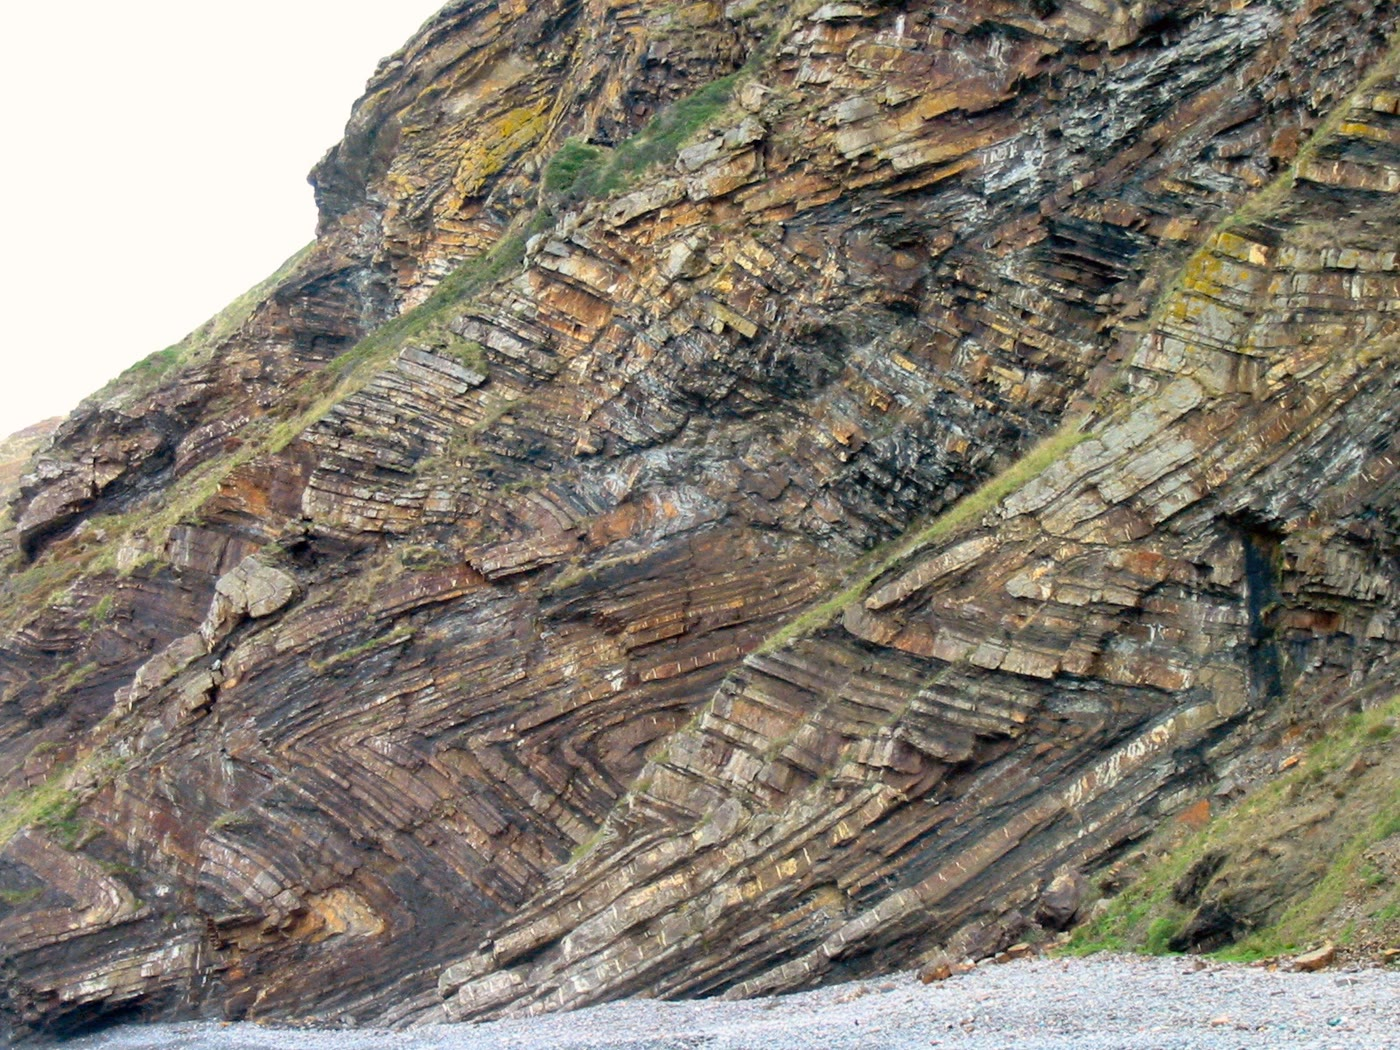
\includegraphics[width=0.78\linewidth]{images/book3/b1-chevron-folds-millook.jpg}
\par\smallskip{\small طبقات مطوية من حجر رملي وصفحي في الجروف عند ميلوك، شمال كورنوال: \omterm{def:b1:geological-maps:fold}{طيّات} شيفرونية ذات \omterm{def:b1:faults-folds-fabrics:fold-elements}{أجنحة} شبه مستقيمة ومفاصل حادّة، ومستوياتها المحورية شبه شاقولية. تصوير: Smalljim, CC~BY~3.0 (ويكيميديا كومنز).}
\label{fig:b1:faults-folds-fabrics:chevrons}
\end{omfigure}
% ledger: commons:millook

\section{النسيج الصخري}\label{sec:b1:faults-folds-fabrics:fabrics}

الصخر المشوّه كثيرًا ما يتشوّه في كامل حجمه، لا على بضعة أسطح فقط: فحبيباته تتفلطح أو تدور أو تُعاد نموّها باتجاه مشترك، فيكتسب نسيجًا. والنسيج المستوي يجعل الصخر ينشقّ، والنسيج الخطّي يجعله ينكسر إلى قضبان.

\begin{definition}[التورّق، والتورّق الشستي، والتشقّق الأردوازي، والتشقّق المحوري المستوي]\label{def:b1:faults-folds-fabrics:foliation}
\emph{التورّق}\index{التورّق} نسيج مستوٍ يعمّ الصخر: مجموعة من الأسطح المتوازية المتقاربة، تتكوّن بحبيبات صفائحية أو مفلطحة مصطفّة أو بطبقات رقيقة، ينشقّ الصخر عليها \omterm{def:b1:faults-folds-fabrics:fault-types}{بأيسر} ما يكون. و\emph{التورّق الشستي}\index{التورّق الشستي} هو تورّق الشست، تكوّنه حبيبات مصطفّة أخشن من نحو \qty{1}{mm}. و\emph{التشقّق}\index{التشقّق (للصخر)} تورّق لصخر دقيق الحبيبات يتكوّن بتشوّهه؛ و\emph{التشقّق الأردوازي}\index{التشقّق الأردوازي} هو تشقّق الأردواز، يتكوّن بسيليكات صفائحية صغيرة جدًّا لا تُرى بالعين المجردة، ومتقاربة إلى حدّ أن الصخر يمكن أن ينشقّ في أيّ مكان تقريبًا إلى صفائح رقيقة. و\emph{التشقّق المحوري المستوي}\index{التشقّق المحوري المستوي} تشقّق يوازي، أو يكاد يوازي، المستويات المحورية \omterm{def:b1:geological-maps:fold}{للطيّات} في الصخور نفسها.
\end{definition}
% ledger: ws:fabrics

يتكوّن \omterm{def:b1:faults-folds-fabrics:foliation}{التورّق} تقريبًا عموديًّا على اتجاه أكبر قصر، بدوران الحبيبات الصفائحية، ونموّ ميكات جديدة، وذوبان الحبيبات على الأوجه الأشدّ ضغطًا. فتشقّق الأردواز لا علاقة له بطبقات الطين التي كان منها: إنه يسجّل الضغط. وحين تنمو \omterm{def:b1:geological-maps:fold}{الطيّات} والتشقّقات في القصر نفسه، يقع \omterm{def:b1:faults-folds-fabrics:foliation}{التشقّق} قريبًا من المستويات المحورية \omterm{def:b1:geological-maps:fold}{للطيّات}، ويتفرّع قليلًا عبرها، متقاربًا أو متباعدًا بحسب قوّة كل طبقة، كما تُظهر الصورة أدناه.
% ledger: ws:fabrics

\begin{omfigure}
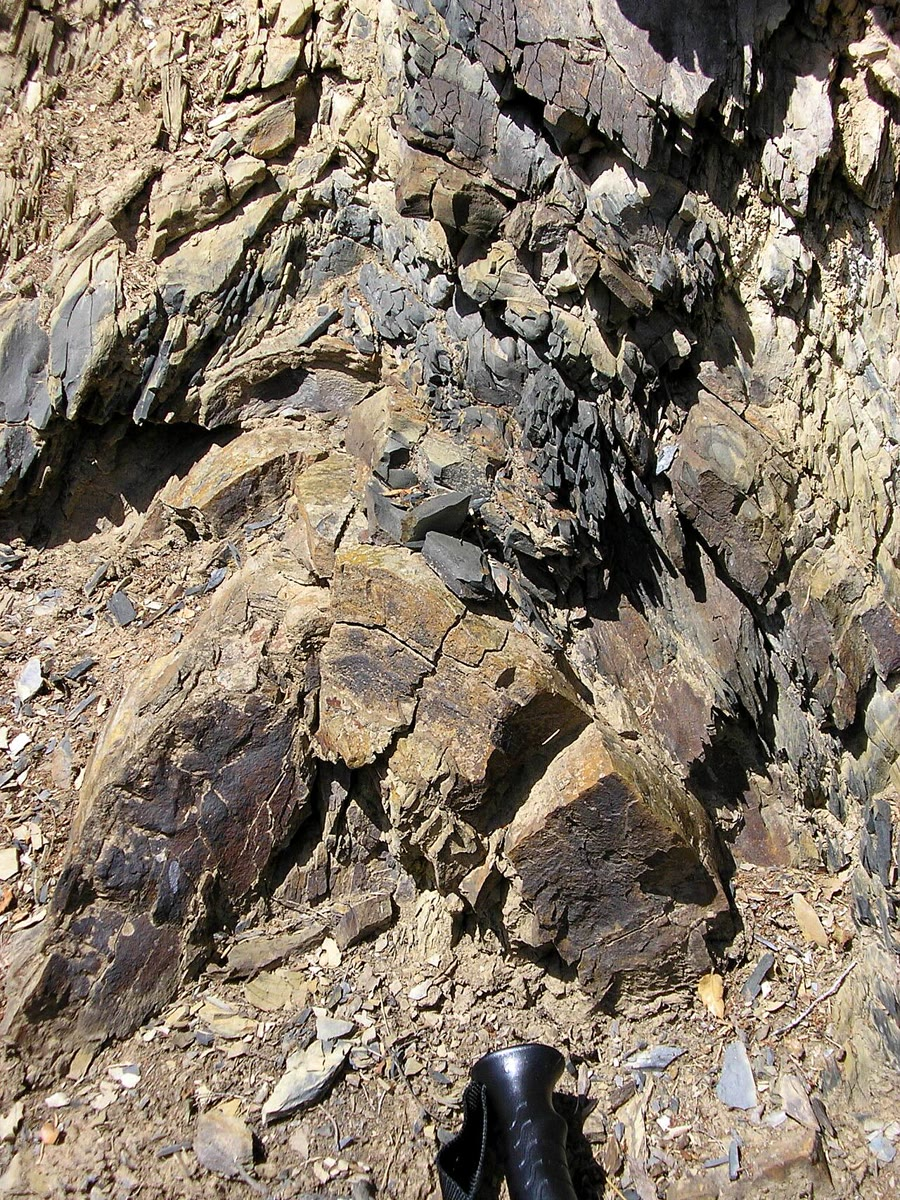
\includegraphics[height=8.2cm]{images/book3/b1-axial-planar-cleavage.jpg}
\par\smallskip{\small \omterm{def:b1:geological-maps:fold}{طيّة} محدّبة صغيرة في تعاقب من حجر رملي وصفحي من عصر الكربوني، قرب بوتيس، كانتابريا. تنحني طبقات الحجر الرملي البنّي فوق \omterm{def:b1:faults-folds-fabrics:fold-elements}{المفصل} في الجزء الأسفل الأوسط من الصورة؛ وفي الصفحي الداكن فوقها يكون \omterm{def:b1:faults-folds-fabrics:foliation}{التشقّق}، مجموعةً من الكسور شديدة الانحدار والمتقاربة تعبر الطبقات، محوريةً مستوية: موازية تقريبًا \omterm{def:b1:faults-folds-fabrics:fold-elements}{للمستوى المحوري} \omterm{def:b1:geological-maps:fold}{للطية}، تتفرّع عبره، وتتغيّر المروحة من طبقة إلى أخرى. ومقبض عصا المشي بعرض نحو \qty{4}{cm}. تصوير: Mikenorton, CC~BY-SA~3.0 (ويكيميديا كومنز).}
\label{fig:b1:faults-folds-fabrics:cleavage}
\end{omfigure}
% ledger: commons:axial-cleavage

\begin{definition}[التخطّط، والتخطّط بالتقاطع، والتخطّط بالاستطالة]\label{def:b1:faults-folds-fabrics:lineation}
\emph{التخطّط}\index{التخطّط} نسيج خطّي يعمّ الصخر، ويُقاس باتجاهه وغوصه. و\emph{التخطّط بالتقاطع}\index{التخطّط بالتقاطع} هو مجموعة الخطوط التي يقطع فيها نسيجان مستويان أحدهما الآخر، كالتطبّق \omterm{def:b1:faults-folds-fabrics:foliation}{والتشقّق}؛ و\emph{التخطّط بالاستطالة}\index{التخطّط بالاستطالة} يتكوّن من حبيبات أو حصى مسحوبة على طول اتجاه أكبر مطّ.
\end{definition}
% ledger: ws:fabrics

\begin{proposition}[التخطّط بالتقاطع لطية]\label{prop:b1:faults-folds-fabrics:intersection}
في \omterm{def:b1:faults-folds-fabrics:fold-elements}{طية أسطوانية} لها تشقّق محوري مستوٍ، يكون \omterm{def:b1:faults-folds-fabrics:lineation}{التخطّط بالتقاطع} للتطبّق مع \omterm{def:b1:faults-folds-fabrics:foliation}{التشقّق} موازيًا \omterm{def:b1:faults-folds-fabrics:fold-elements}{لخطّ المفصل}، في كل مكان من \omterm{def:b1:geological-maps:fold}{الطية}.
\end{proposition}

\begin{proof}
يحتوي كل سطح تطبّق \omterm{def:b1:faults-folds-fabrics:fold-elements}{لطية أسطوانية} اتجاه محورها. \omterm{def:b1:faults-folds-fabrics:fold-elements}{والمستوى المحوري} يحتوي خطوط المفاصل، الموازية للمحور، فيحتوي ذلك الاتجاه أيضًا، وكذلك كل مستوى تشقّق موازٍ له. والمستويان غير المتوازيين اللذان يحتويان الاتجاه نفسه يتقاطعان على خطّ من ذلك الاتجاه.
\end{proof}

وهذه القضية هي طريق الجيولوجي الميداني إلى غوص \omterm{def:b1:geological-maps:fold}{طية} أكبر من أن تُرى كاملةً: فعلى أيّ \omterm{def:b1:geological-maps:geological-map}{انكشاف} لأحد الجناحين، تعطي الخطوط التي يقطع فيها \omterm{def:b1:faults-folds-fabrics:foliation}{التشقّق} التطبّق \omterm{def:b1:faults-folds-fabrics:fold-elements}{خطّ المفصل}. والتطبّق \omterm{def:b1:faults-folds-fabrics:foliation}{والتشقّق} معًا يقولان أكثر: أين تقع \omterm{def:b1:geological-maps:fold}{الطية}، وأيّ الجهات أعلى الطبقات.

\begin{definition}[الاتجاه الانقلابي]\label{def:b1:faults-folds-fabrics:vergence}
\emph{الاتجاه الانقلابي}\index{الاتجاه الانقلابي} \omterm{def:b1:geological-maps:fold}{لطيّة} غير متماثلة هو الاتجاه الأفقي الذي تحرّك نحوه جزؤها العلوي بالنسبة لجزئها السفلي: الاتجاه الذي تنقلب نحوه، أو، بالنسبة \omterm{def:b1:faults-folds-fabrics:fold-classes}{لطيّة مائلة}، الاتجاه الذي تميل نحوه.
\end{definition}
% ledger: ws:vergence

\begin{proposition}[التطبّق والتشقّق على أجنحة الطية]\label{prop:b1:faults-folds-fabrics:cleavage-bedding}
لتكن \omterm{def:b1:geological-maps:fold}{طية} لها \omterm{def:b1:faults-folds-fabrics:fold-elements}{أجنحة} مستقيمة وتشقّق محوري مستوٍ، في صخور كانت في وضعها الصحيح قبل الطيّ، وينزل فيها الجناحان من كل \omterm{def:b1:geological-maps:fold}{طية} محدّبة مفصل. وفي المقطع:
\begin{enumerate}[label=(\alph*)]
  \item على جناح ينحدر فيه التطبّق \omterm{def:b1:faults-folds-fabrics:foliation}{والتشقّق} بالاتجاه نفسه، يكون التطبّق أشدّ انحدارًا من \omterm{def:b1:faults-folds-fabrics:foliation}{التشقّق} تحديدًا حين يكون الجناح منقلبًا؛
  \item الدوران الحادّ الذي يدير \omterm{def:b1:faults-folds-fabrics:foliation}{التشقّق} إلى التطبّق له اتجاهان متعاكسان على جناحي \omterm{def:b1:geological-maps:fold}{الطية}؛ فعلى جناح غير منقلب، يحرّك أعلى \omterm{def:b1:faults-folds-fabrics:foliation}{التشقّق} أفقيًّا نحو \omterm{def:b1:faults-folds-fabrics:fold-elements}{المفصل} المحدّب الواقع أعلى ذلك الجناح.
\end{enumerate}
\end{proposition}

\begin{proof}
انظر على طول \omterm{def:b1:faults-folds-fabrics:fold-elements}{المفصل} \omterm{def:b1:faults-folds-fabrics:fold-elements}{والمستوى المحوري} ينحدر نحو اليسار بالزاوية
$\gamma$، $0 < \gamma \le \ang{90}$، وعُدَّ الزوايا عكس عقارب الساعة من الأفقي المتّجه نحو اليمين. \omterm{def:b1:faults-folds-fabrics:foliation}{والتشقّق}، الموازي \omterm{def:b1:faults-folds-fabrics:fold-elements}{للمستوى المحوري}، يصعد بالزاوية $\gamma$. وعند مفصل محدّب يخرج الجناحان نحو الأسفل بالزاويتين $\ang{180} + \gamma - \iota/2$ (الجناح~1) و$\ang{180} + \gamma + \iota/2$ (الجناح~2)، على جانبي \omterm{def:b1:faults-folds-fabrics:fold-elements}{المستوى المحوري}، مع $\iota/2 \le \gamma$ لأن كليهما ينزل؛ وكل جناح في سلسلة من \omterm{def:b1:geological-maps:fold}{الطيّات} هو أحد هذين \omterm{def:b1:geological-maps:fold}{للطية} المحدّبة التي فوقه. وتصبح الطبقات أحدث عمرًا نحو الخارج، بعيدًا عن لبّ \omterm{def:b1:geological-maps:fold}{الطية} المحدّبة، على طول العمودي على الجناح الذي يشير بعيدًا عن \omterm{def:b1:faults-folds-fabrics:fold-elements}{المستوى المحوري}.

الجناح~1 ينزل نحو اليسار: ينحدر نحو اليسار بالزاوية $\gamma - \iota/2$، أقلّ شدّة من \omterm{def:b1:faults-folds-fabrics:foliation}{التشقّق}. وعموده الخارجي، عند $\ang{90} + \gamma -
\iota/2$، يشير إلى الأعلى: فهو في وضعه الصحيح. وبالصعود فيه يصنع الزاوية $\gamma - \iota/2$، فيكون الدوران الحادّ من \omterm{def:b1:faults-folds-fabrics:foliation}{التشقّق} إلى التطبّق مع عقارب الساعة، عبر $\iota/2$: فيتحرّك أعلى \omterm{def:b1:faults-folds-fabrics:foliation}{التشقّق} نحو اليمين، حيث يقع \omterm{def:b1:faults-folds-fabrics:fold-elements}{المفصل}، لأن الجناح يخرج من \omterm{def:b1:faults-folds-fabrics:fold-elements}{المفصل} نحو اليسار.

الجناح~2 يصنع الزاوية $\gamma + \iota/2$ مع الأفقي، صاعدًا. فإن كانت $\gamma + \iota/2 > \ang{90}$، ينزل نحو اليمين وينحدر نحو اليمين، عكس \omterm{def:b1:faults-folds-fabrics:foliation}{التشقّق}؛ وعموده الخارجي، عند $\ang{270} + \gamma +
\iota/2$، له المركّبة الصاعدة $-\cos(\gamma + \iota/2) > 0$: فهو في وضعه الصحيح. وإن كانت $\gamma + \iota/2 < \ang{90}$، ينزل نحو اليسار، منحدرًا نحو اليسار بالزاوية $\gamma + \iota/2$، أشدّ من \omterm{def:b1:faults-folds-fabrics:foliation}{التشقّق}، وتكون المركّبة نفسها سالبة: فالجناح منقلب. وفي الحالتين يكون الدوران الحادّ من \omterm{def:b1:faults-folds-fabrics:foliation}{التشقّق} إلى التطبّق عكس عقارب الساعة، عبر $\iota/2$، ويحرّك أعلى \omterm{def:b1:faults-folds-fabrics:foliation}{التشقّق} نحو اليسار؛ وحين يكون الجناح في وضعه الصحيح يترك \omterm{def:b1:faults-folds-fabrics:fold-elements}{المفصل} نحو اليمين، فيكون \omterm{def:b1:faults-folds-fabrics:fold-elements}{المفصل} إلى اليسار. \omterm{def:b1:faults-folds-fabrics:fold-elements}{فالأجنحة} التي تنحدر بالاتجاه نفسه الذي ينحدر به \omterm{def:b1:faults-folds-fabrics:foliation}{التشقّق} هي إذن الجناح~1، الأقلّ شدّة، والجناح~2 المنقلب، الأشدّ، وهو الحالة (أ)؛ والاتجاهان مع عقارب الساعة على الجناح~1 وعكسها على الجناح~2، وهو الحالة (ب).
\end{proof}

وهكذا يتغيّر اتجاه الدوران عند كل مفصل، محدّب أو مقعّر.
والجيولوجي الذي يسجّله على امتداد مسار يجد أن مفاصل \omterm{def:b1:geological-maps:fold}{الطيّات} أكبر من أن تُرى في \omterm{def:b1:geological-maps:geological-map}{انكشاف} واحد حيث يتغيّر الاتجاه، \omterm{def:b1:faults-folds-fabrics:fold-elements}{والأجنحة} المنقلبة حيث يكون التطبّق أشدّ انحدارًا من \omterm{def:b1:faults-folds-fabrics:foliation}{التشقّق}؛ ويُستعمل لفظ \omterm{def:b1:faults-folds-fabrics:vergence}{الاتجاه الانقلابي} لهذا الاتجاه من الدوران أيضًا، وتُرسم انعكاسات \omterm{def:b1:faults-folds-fabrics:vergence}{الاتجاه الانقلابي} \omterm{def:b1:geological-maps:fold}{للطيّات} الصغرى بالطريقة نفسها لإيجاد مفاصل \omterm{def:b1:geological-maps:fold}{الطيّات} الكبرى: \omterm{def:b1:geological-maps:fold}{فالطيّات} الصغيرة على جناحي \omterm{def:b1:geological-maps:fold}{طية} كبيرة لها لاتماثلات متعاكسة، وأثرها المحوري يمرّ بينهما.
% ledger: ws:vergence, ws:fold-elements

\begin{omfigure}
\begin{tikzpicture}[>={Stealth[length=5pt]}, font=\small]
% a train of chevron folds seen along the hinge (north into the page, east to the right):
% axial planes dipping 60 deg to the west, interlimb angle 40 deg; long limbs dip 40 deg W
% (the right way up), short limbs 80 deg W (overturned). Short limb: from an anticline hinge H_k,
% length s along 260 deg to the syncline hinge S_k; long limb back up along 40 deg to H_{k+1},
% so that all anticline hinges are level, a wavelength w apart.
% Five bedding surfaces, repeated along the axial direction (similar folds); cleavage parallel to it.
\def\s{2.6}
\pgfmathsetmacro{\sx}{\s*cos(260)}\pgfmathsetmacro{\sy}{\s*sin(260)}
\pgfmathsetmacro{\w}{\sx - \sy/tan(40)}
\pgfmathsetmacro{\hx}{0.62*cos(60)}\pgfmathsetmacro{\hy}{0.62*sin(60)}
\newcommand{\surface}[1]{%
  (-\w+#1*\hx, #1*\hy) \foreach \k in {-1,0,1,2,3} { -- ({\k*\w+\sx+#1*\hx}, {\sy+#1*\hy}) -- ({(\k+1)*\w+#1*\hx}, {#1*\hy}) }}
\begin{scope}
  \clip (0.35,-3.3) rectangle (10.0,2.95);
  \begin{scope}
    \clip \surface{0} -- (12,6) -- (-4,6) -- cycle;
    \clip \surface{4} -- (12,-6) -- (-4,-6) -- cycle;
    \fill[omLithSand!45] (-4,-6) rectangle (12,6);
    \fill[omLithShale!40] \surface{2} -- (12,6) -- (-4,6) -- cycle;
    \fill[omLithSand!45] \surface{3} -- (12,6) -- (-4,6) -- cycle;
    \foreach \c in {-8.0,-7.78,...,13.0} {
      \draw[omDef!85, line width=0.35pt] ({\c-6*cot(60)},-6) -- ({\c+6*cot(60)},6);
    }
  \end{scope}
  \foreach \j in {0,1,2,3,4} { \draw[line width=0.75pt, line join=round] \surface{\j}; }
\end{scope}
% axial traces through the anticline hinges, and labels
\foreach \k in {1,2,3} {
  \draw[omThm, dashed, line width=0.6pt] ({\k*\w-0.5*cos(60)},{-0.5*sin(60)}) -- ({\k*\w+3.6*cos(60)},{3.6*sin(60)});
  \node[omThm, font=\scriptsize, anchor=south] at ({\k*\w+3.6*cos(60)},{3.6*sin(60)}) {طية محدّبة};
}
\foreach \k in {1,2,3} { \node[omThm, font=\scriptsize, anchor=north] at ({\k*\w+\sx},{\sy-0.15}) {طية مقعّرة}; }
\end{tikzpicture}
\par\smallskip{\small سلسلة من \omterm{def:b1:geological-maps:fold}{الطيّات} الشيفرونية منقلبة نحو اليمين، في المقطع، مع تشقّق محوري مستوٍ (خطوط زرقاء رفيعة)، مرسومة بالمقياس: المستويات المحورية ينحدر بزاوية \ang{60} نحو اليسار، \omterm{def:b1:faults-folds-fabrics:fold-elements}{وزاوية الأجنحة} \ang{40}. \omterm{def:b1:faults-folds-fabrics:fold-elements}{والأجنحة} الطويلة ينحدر \ang{40} نحو اليسار، أقلّ شدّة من \omterm{def:b1:faults-folds-fabrics:foliation}{التشقّق}، وهي في وضعها الصحيح؛ \omterm{def:b1:faults-folds-fabrics:fold-elements}{والأجنحة} القصيرة تنحدر \ang{80} نحو اليسار، أشدّ من \omterm{def:b1:faults-folds-fabrics:foliation}{التشقّق}، وهي منقلبة. والدوران الذي يُدير \omterm{def:b1:faults-folds-fabrics:foliation}{التشقّق} إلى التطبّق عبر الزاوية الحادّة يكون مع عقارب الساعة على كل جناح طويل، وعكسها على كل جناح قصير. وتنقلب \omterm{def:b1:geological-maps:fold}{الطيّات} نحو اليمين.}
\label{fig:b1:faults-folds-fabrics:vergence}
\end{omfigure}

\section{البنيات المجهرية}\label{sec:b1:faults-folds-fabrics:micro}

تحت المجهر يظهر تشوّه الصخر في حبيباته. فحبّة كوارتز انحنت بانزلاق بطيء لشبيكتها البلورية لم تعد تنطفئ دفعة واحدة بين \omterm{def:b1:field-lab-methods-1:microscope}{المستقطِبين المتقاطعين}: فحين تدور المنضدة يمرّ نطاق داكن عبرها، لأن أجزاءها تشير إلى اتجاهات مختلفة قليلًا. وهذا الانطفاء المتموّج (\cref{ch:b1:optical-mineralogy}) يشتدّ كلما اقترب المرء من منطقة قصّ، لأن العيوب تتراكم في الشبيكة البلورية. وحيث يوجد الماء، تذوب الحبيبات على الأوجه الأشدّ ضغطًا، فتترسّب المادة المذابة حيث الإجهاد أدنى، أو تُحمل بعيدًا: وهذا الذوبان بالضغط يقصّر الصخور في حرارة منخفضة، ويبني تشقّقات كثيرة. وعند حرارة أعلى، تُستبدل الحبيبات المجهدة، بينما يستمرّ التشوّه، بحبيبات جديدة أصغر وغير مجهدة، أولًا على حدود الحبيبات القديمة: إعادة التبلور الديناميكية، التي تُصغّر حجم الحبيبات وتكوّن الميلونيتات. وأشكال الحبيبات المشوّهة \omterm{def:b1:rock-forming-minerals:mineral}{والمعادن} التي تنمو في ظلالها تبيّن أيضًا في أيّ اتجاه تحرّكت منطقة القصّ؛ وهذه مؤشرات اتجاه القصّ، وآلياتها أنفسها، من اختصاص مجلد السنة الثالثة.
% ledger: ws:microstructures, ws:fabrics

\section{التمارين}

\begin{exercise}[$\star$]\label{exo:b1:faults-folds-fabrics:1}
سمِّ كل صدع من زاوية انزلاق متجهة انزلاقه، والمستوى ينحدر \ang{60}:
(أ) $r = \ang{-90}$؛ (ب) $r = \ang{85}$؛ (ج) $r = 0$؛ (د) $r = \ang{180}$؛
(ه) $r = \ang{-40}$. (و) بماذا يُسمّى (ب) لو كان انحداره \ang{25}؟
% ledger: ar:rake, usgs:fault-types
\end{exercise}

\begin{exercise}[$\star$]\label{exo:b1:faults-folds-fabrics:2}
\omterm{def:b1:faults-folds-fabrics:fault-types}{صدع عادي} ينحدر \ang{55}؛ انزلاقه شاقولي خالص، مع انزلاق صافٍ قدره \qty{300}{m}. احسب إزاحته الرأسية \omterm{def:b1:cross-sections:throw}{وإزاحته الأفقية}.
\end{exercise}

\begin{exercise}[$\star$]\label{exo:b1:faults-folds-fabrics:3}
أعطِ \omterm{def:b1:faults-folds-fabrics:fold-elements}{زاوية الأجنحة} وصنف كل \omterm{def:b1:faults-folds-fabrics:fold-classes}{طية قائمة}، يكون جناحاها ينحدران في اتجاهين متعاكسين: (أ) جناحان ينحدران \ang{35} و\ang{35}؛ (ب) \ang{70} و\ang{75}؛ (ج) \ang{85} و\ang{88}.
% ledger: ws:fold-classes
\end{exercise}

\begin{exercise}[$\star$]\label{exo:b1:faults-folds-fabrics:4}
صخر رملي له \omterm{def:b1:stress-strain-rheology:coulomb}{زاوية الاحتكاك الداخلي} \ang{35}. وفق نظرية أندرسون، بأيّ زوايا تنحدر صدوعه العادية والدفعية؟ وما الزاوية التي يصنعها صدعان انزياحيان مترافقان مع بعضهما؟
\end{exercise}

\begin{exercise}[$\star\star$]\label{exo:b1:faults-folds-fabrics:5}
لصدع \omterm{def:b1:geological-maps:attitude}{وضعية} $090/50$، وخدوش منزلقة عليه من زاوية انزلاق \ang{-30}؛ \omterm{def:b1:faults-folds-fabrics:fault-elements}{والانزلاق الصافي} \qty{400}{m}. (أ) احسب مركّبتي الانزياح والانزلاق الشاقولي، \omterm{def:b1:cross-sections:throw}{والإزاحة الرأسية} \omterm{def:b1:cross-sections:throw}{والإزاحة الأفقية}. (ب) اكتب \omterm{def:b1:faults-folds-fabrics:fault-elements}{متجهة الانزلاق} بمركّبات شرقية وشمالية وعلوية، وأعطِ اتجاهها وغوصها. (ج) سمِّ الصدع.
\end{exercise}

\begin{exercise}[$\star\star$]\label{exo:b1:faults-folds-fabrics:6}
صدعان انزياحيان شاقوليان من العمر نفسه، امتدادهما $020$ و$080$. (أ) وفق أندرسون، أعطِ اتجاهات $\sigma_1$ و$\sigma_2$ و$\sigma_3$، \omterm{def:b1:stress-strain-rheology:coulomb}{وزاوية الاحتكاك الداخلي} للصخر. (ب) أيّ الصدعين \omterm{def:b1:faults-folds-fabrics:fault-types}{أيمن} وأيّهما \omterm{def:b1:faults-folds-fabrics:fault-types}{أيسر}؟ استدلّ بالقصر على طول $\sigma_1$.
\end{exercise}

\begin{exercise}[$\star\star$]\label{exo:b1:faults-folds-fabrics:7}
لطرفي \omterm{def:b1:faults-folds-fabrics:fold-elements}{طية أسطوانية} وضعيتان $120/40$ و$260/30$. وباستعمال \cref{prop:b1:faults-folds-fabrics:hinge}، أوجد اتجاه وغوص خطّ مفصلها، وزاوية أجنحتها، وصنفها.
\end{exercise}

\begin{exercise}[$\star\star$]\label{exo:b1:faults-folds-fabrics:8}
عند \omterm{def:b1:geological-maps:geological-map}{انكشاف}، للتطبّق \omterm{def:b1:geological-maps:attitude}{وضعية} $040/30$، وللتشقّق المحوري المستوي \omterm{def:b1:geological-maps:attitude}{وضعية} $160/80$. أوجد اتجاه وغوص \omterm{def:b1:faults-folds-fabrics:lineation}{التخطّط بالتقاطع}. ماذا يخبرنا عن \omterm{def:b1:geological-maps:fold}{الطية}؟
\end{exercise}

\begin{exercise}[$\star\star$]\label{exo:b1:faults-folds-fabrics:9}
صدع شاقولي يمتدّ شرق--غرب. يقطعه عِرق صخري شاقولي يمتدّ شمال--جنوب؛ شمال الصدع يوجد العِرق على بعد \qty{350}{m} شرق المكان الذي يقع فيه جنوبه. (أ) هل الصدع \omterm{def:b1:faults-folds-fabrics:fault-types}{أيمن} أم \omterm{def:b1:faults-folds-fabrics:fault-types}{أيسر}؟ (ب) إذا كانت \omterm{def:b1:faults-folds-fabrics:fault-rocks}{الخدوش المنزلقة} أفقية، فما \omterm{def:b1:faults-folds-fabrics:fault-elements}{الانزلاق الصافي}؟ (ج) وإذا كانت بدلًا من ذلك تغوص \ang{20} نحو الشرق، فما \omterm{def:b1:faults-folds-fabrics:fault-elements}{الانزلاق الصافي} ومركّبة الانزلاق الشاقولي، وأيّ الكتلتين نزلت؟
\end{exercise}

\begin{exercise}[$\star\star\star$]\label{exo:b1:faults-folds-fabrics:10}
صدع بلا تماسك، ومعامل احتكاك $\mu$، يصنع الزاوية $\theta$ مع $\sigma_1$. (أ) بيّن أنه ينزلق حين تبلغ \omterm{def:b1:stress-strain-rheology:principal}{الإجهادات الرئيسية} الفعّالة النسبة
\[
  \frac{\sigma_1'}{\sigma_3'} = \frac{1 + \mu\cot\theta}{1 - \mu\tan\theta} .
\]
(ب) مع $\mu = 0.6$ و$\sigma_1$ شاقوليًّا، احسب النسبة للصدوع العادية التي تنحدر \ang{60} و\ang{45} و\ang{35}. (ج) بيّن أن صدعًا عاديًّا ينحدر بأقلّ من زاوية معيّنة لا ينزلق أبدًا، واحسب تلك الزاوية. (د) من أجل $\mu = 0.6$ و$\mu = 0.85$، أعطِ انحدارات أفضل الصدوع العادية والدفعية توجّهًا.
\end{exercise}

\begin{exercise}[$\star\star\star$]\label{exo:b1:faults-folds-fabrics:11}
على امتداد شرق--غرب عبر \omterm{def:b1:geological-maps:fold}{طيّات} شيفرونية مفاصلها تتّجه شمالًا، تشقّق محوري مستوٍ ينحدر \ang{60} نحو الغرب في كل مكان. ينحدر التطبّق \ang{40} غربًا عند المحطة A، و\ang{80} غربًا عند المحطة B، و\ang{40} غربًا عند المحطة C، من الغرب إلى الشرق، في صخور كانت في وضعها الصحيح قبل الطيّ. (أ) أيّ المحطات تقع على جناح منقلب؟ (ب) في أيّ اتجاه يدور \omterm{def:b1:faults-folds-fabrics:foliation}{التشقّق} ليصبح على التطبّق عند كل محطة، عند النظر شمالًا؟ (ج) أين تقع المفاصل، وأيّها \omterm{def:b1:geological-maps:fold}{طيّات} محدّبة؟ (د) أوجد \omterm{def:b1:faults-folds-fabrics:fold-elements}{زاوية الأجنحة} \omterm{def:b1:geological-maps:attitude}{ووضعية} المستويات المحورية، وقُل في أيّ اتجاه تنقلب \omterm{def:b1:geological-maps:fold}{الطيّات}.
\end{exercise}

\begin{exercise}[$\star\star\star$]\label{exo:b1:faults-folds-fabrics:12}
يُطوى طول $L_0$ من طبقة إلى سلسلة من \omterm{def:b1:geological-maps:fold}{طيّات} شيفرونية متماثلة، زاوية أجنحتها $\iota$، مع بقاء طوله دون تغيير. (أ) بيّن أن طوله مقيسًا عبر \omterm{def:b1:geological-maps:fold}{الطيّات} يصبح $L_0\sin(\iota/2)$. (ب) أيّ قصر تمثّل \omterm{def:b1:geological-maps:fold}{طيّات} شيفرونية زاوية أجنحتها \ang{60}؟ (ج) أيّ \omterm{def:b1:faults-folds-fabrics:fold-elements}{زاوية أجنحة} توافق قصرًا قدره \qty{30}{\percent}؟ (د) سلسلة من \omterm{def:b1:geological-maps:fold}{الطيّات} القائمة أجنحتها تنحدر \ang{12}: ما القصر؟
\end{exercise}

\section{مسألة: بنيات تلال فاردن، مقاسةً}

\begin{problem}[{مسألة نهاية الأسبوع: الطية المحدّبة والصدع العادي في تلال فاردن، من وضعيات مستوياتها إلى انزلاق الصدع}]
\label{pb:b1:faults-folds-fabrics:1}
% values: calc/ch17.py; region: figdata/shared/region.py (limbs, plunge, fault)
تلال فاردن مطوية في \omterm{def:b1:geological-maps:fold}{طية} محدّبة، يمتدّ محورها شمال--جنوب عند $x = \qty{3.5}{km}$، وفي \omterm{def:b1:geological-maps:fold}{طية} مقعّرة على بُعد \qty{4}{km} شرقها؛ ولكلتيهما \omterm{def:b1:faults-folds-fabrics:fold-elements}{أجنحة} مستوية. وقد قاس مسح ميداني التطبّق على الجناح الشرقي \omterm{def:b1:geological-maps:fold}{للطية} المحدّبة \omterm{def:b1:geological-maps:attitude}{بوضعية} $080.7/12.2$، وعلى جناحها الغربي \omterm{def:b1:geological-maps:attitude}{بوضعية} $279.3/12.2$. ويقطع الغطاء \omterm{def:b1:faults-folds-fabrics:fault-types}{صدع عادي} وضعيته $120/60$، ينزل فيه \omterm{def:b1:faults-folds-fabrics:fault-elements}{الجدار المعلّق} على طول \omterm{def:b1:geological-maps:attitude}{الانحدار}، وإزاحته الرأسية \qty{200}{m}. أعطِ الزوايا حتى \ang{0.1} والأطوال حتى \qty{0.1}{m}.

\medskip
\noindent\textbf{الجزء الأول --- \omterm{def:b1:faults-folds-fabrics:fold-elements}{الأجنحة}.}
\begin{enumerate}
  \item اكتب المتجهتين الوحدتين العموديتين العلويتين $\mathbf n_1$ (الجناح الشرقي) و$\mathbf n_2$ (الجناح الغربي) بمركّبات شرقية وشمالية وعلوية.
  \item احسب $\mathbf n_1\cdot\mathbf n_2$ والزاوية بين العموديين.
  \item استنتج \omterm{def:b1:faults-folds-fabrics:fold-elements}{زاوية الأجنحة} \omterm{def:b1:geological-maps:fold}{للطية} المحدّبة.
  \item صنّف \omterm{def:b1:geological-maps:fold}{الطية} المحدّبة بحسب زاوية أجنحتها.
  \item ينحدر الجناحان بالزاوية \ang{12.2}. لماذا لا تساوي \omterm{def:b1:faults-folds-fabrics:fold-elements}{زاوية الأجنحة} بالضبط $\ang{180} - 2\times\ang{12.2}$؟ واحسب \omterm{def:b1:cross-sections:apparent-dip}{الانحدار الظاهري} لأيّ من الجناحين في مقطع شاقولي شرق--غرب.
  \item تشارك \omterm{def:b1:geological-maps:fold}{الطية} المقعّرة الجناح الشرقي \omterm{def:b1:geological-maps:fold}{للطية} المحدّبة، وجناحها الشرقي موازٍ لجناح \omterm{def:b1:geological-maps:fold}{الطية} المحدّبة الغربي. ما زاوية أجنحتها؟
\end{enumerate}

\medskip
\noindent\textbf{الجزء الثاني --- \omterm{def:b1:faults-folds-fabrics:fold-elements}{خطّ المفصل} \omterm{def:b1:faults-folds-fabrics:fold-elements}{والمستوى المحوري}.}
\begin{enumerate}[resume]
  \item احسب $\mathbf n_1\times\mathbf n_2$، والاتجاه \omterm{def:b1:field-lab-methods-1:trend-plunge}{والغوص} \omterm{def:b1:faults-folds-fabrics:fold-elements}{لخطّ المفصل}.
  \item أعطِ \omterm{def:b1:geological-maps:attitude}{وضعية} \omterm{def:b1:faults-folds-fabrics:fold-elements}{المستوى المحوري}. هل \omterm{def:b1:geological-maps:fold}{الطية} المحدّبة قائمة أم مائلة أم مستلقية؟
  \item أعطِ وصفًا كاملًا \omterm{def:b1:geological-maps:fold}{للطية}: الإحكام، \omterm{def:b1:geological-maps:attitude}{ووضعية} \omterm{def:b1:faults-folds-fabrics:fold-elements}{المستوى المحوري}، \omterm{def:b1:field-lab-methods-1:trend-plunge}{والغوص}.
  \item على \omterm{def:b1:geological-maps:geological-map}{الخريطة الجيولوجية} في \cref{ch:b1:geological-maps}، كيف تقترب \omterm{def:b1:geological-maps:geological-map}{انكشافات} \omterm{def:b1:geological-maps:fold}{الطية} المحدّبة من بعضها، وماذا يظهر في لبّها؟
  \item يحمل صفيح الغطاء تشقّقًا محوريًّا مستويًّا. أعطِ وضعيته، والاتجاه \omterm{def:b1:field-lab-methods-1:trend-plunge}{والغوص} لتخطّطه بالتقاطع على الجناح الشرقي.
  \item على الجناح الشرقي، في أيّ اتجاه يدور \omterm{def:b1:faults-folds-fabrics:foliation}{التشقّق} ليصبح على التطبّق، عند النظر شمالًا، وعلى أيّ جانب يقع مفصل \omterm{def:b1:geological-maps:fold}{الطية} المحدّبة؟
\end{enumerate}

\medskip
\noindent\textbf{الجزء الثالث --- الصدع والإجهادات.}
\begin{enumerate}[resume]
  \item أعطِ امتداد الصدع بقاعدة اليد اليمنى، وقُل على أيّ جانب من أثره يقع \omterm{def:b1:faults-folds-fabrics:fault-elements}{الجدار المعلّق}.
  \item أيّ \omterm{def:b1:stress-strain-rheology:principal}{الإجهادات الرئيسية} كان شاقوليًّا حين تكوّن الصدع، وفق أندرسون؟
  \item أعطِ اتجاهي الإجهادين الرئيسيين الأفقيين.
  \item ما \omterm{def:b1:stress-strain-rheology:coulomb}{زاوية الاحتكاك الداخلي} التي يقتضيها \omterm{def:b1:geological-maps:attitude}{الانحدار}؟ وما \omterm{def:b1:stress-strain-rheology:coulomb}{معامل الاحتكاك الداخلي}؟
  \item أعطِ \omterm{def:b1:geological-maps:attitude}{وضعية} المجموعة المترافقة من الصدوع التي يمكن أن تكون الإجهادات نفسها قد كوّنتها، والزاوية بين المجموعتين.
  \item هل سيكون الصدع أفضل توجّهًا للانزلاق مجددًا تحت النظام نفسه، مع احتكاك بايرلي 0.85؟
\end{enumerate}

\medskip
\noindent\textbf{الجزء الرابع --- الانزلاق.}
\begin{enumerate}[resume]
  \item أعطِ \omterm{def:b1:faults-folds-fabrics:fault-elements}{زاوية الانزلاق} \omterm{def:b1:faults-folds-fabrics:fault-elements}{لمتجهة الانزلاق}، واتجاهها وغوصها.
  \item اكتب متجهة الوحدة للانزلاق بمركّبات شرقية وشمالية وعلوية.
  \item احسب \omterm{def:b1:cross-sections:throw}{الإزاحة الأفقية} للصدع.
  \item احسب المركّبتين الشرقية والشمالية \omterm{def:b1:cross-sections:throw}{للإزاحة الأفقية} \omterm{def:b1:faults-folds-fabrics:fault-elements}{للجدار المعلّق}.
  \item تحقّق أن \omterm{def:b1:faults-folds-fabrics:fault-elements}{الانزلاق الصافي} $L$ \omterm{def:b1:cross-sections:throw}{والإزاحة الرأسية} $h$ \omterm{def:b1:cross-sections:throw}{والإزاحة الأفقية} $e$ تحقّق $L^2 = h^2 + e^2$، واشرح لماذا.
  \item لأقرب متر، ما \omterm{def:b1:faults-folds-fabrics:fault-elements}{الانزلاق الصافي} على صدع فاردن؟
\end{enumerate}
\end{problem}
